% #####################################################
% Alida Manual
%
% File:               AlidaManual.tex
% Author:             Stefan Posch / Birgit Moeller
% Date:               08.04.2011
% last update:        February 2015
% #####################################################

\documentclass[twoside,11pt,a4paper,english]{article}

\usepackage{amsmath}                   %% mathmatical symbols and formulas
\usepackage[english]{babel}             %% german special signs
\usepackage{epsfig}
\usepackage{fancyheadings}             %% headings and footer
\usepackage{graphics}                  %% inclusion of graphics
\usepackage{graphicx}                  %%     "       "      "
\usepackage{listings}
\usepackage{color}
\usepackage{subfigure}
\usepackage{framed}
\usepackage{url}
\usepackage{hyperref}
\usepackage{xspace}
\usepackage{wrapfig} 

\newcommand{\alida}{{\bf \tt Alida}\xspace}
\newcommand{\mitobo}{{\bf \tt MiToBo}\xspace}
\newcommand{\grappa}{{\bf \tt Grappa}\xspace}
\newcommand{\mtbimg}{\texttt{MTBImage}}
\newcommand{\imgplus}{\texttt{ImagePlus}}
\newcommand{\imgproc}{\texttt{ImageProcessor}}
\newcommand{\mtbc}{{\bf \tt Chipory}\xspace}
\newcommand{\chipo}{{\bf \tt Chipory}\xspace}
\newcommand{\chipory}{{\bf \tt Chipory}\xspace}

\newcommand{\TODO}[1]{\textcolor{red}{TODO:} \textit{#1}}
\renewcommand{\TODO}[1]{}

%%%% layout
\newcommand{\itemseparation}[1]{\parskip#1\topsep#1\partopsep#1%
    \parsep#1\itemsep#1}

%%%% lstlisting
\lstset{language=Java, columns=flexible, tabsize=2, numbers=left}

%% inline code
\newcommand{\icode}[1]{\lstinline[language=Clean]{#1}}
\renewcommand{\icode}[1]{\texttt{#1}}

\newcommand{\demoCodeDir}{../codeSnippets}

\lstnewenvironment{code}
  {~\\\noindent
   \minipage{\linewidth} 
   \vspace{0.5\baselineskip}
\lstset{language=java,numbers=none,frame=single}}
  {\endminipage\\}

\lstnewenvironment{codecsh}
  {~\\\noindent
   \minipage{\linewidth} 
   \vspace{0.5\baselineskip}
\lstset{language=csh,numbers=none,frame=single}}
  {\endminipage\\}

% graphics path
\graphicspath{{../images/}}

% margins
\evensidemargin = -0.5cm
\oddsidemargin = 0.0cm

\textheight 23cm 
\textwidth 16cm
\topmargin -0.75cm
\headsep 1cm
\footskip 1.5cm

%\parindent0pt                          %% no indent of new paragraphs
\renewcommand{\baselinestretch}{1.2}   %% big lineskips

\frenchspacing                         
\sloppy                                %% newlines

\setcounter{tocdepth}{3}               %% depth of table of contents

\setlength\parskip{\medskipamount}     %% line skippings
\parskip1.5ex plus 0.5ex minus 0.5ex   %%

% standard headings and footer
\renewcommand{\sectionmark}[1]{\markboth{\thesection\ #1}{}}
\renewcommand{\sectionmark}[1]{\markleft{\thesection\ #1}{}}

\pagestyle{fancy}
\lhead[\fancyplain{}{}]{\fancyplain{}{}}
\rhead[\fancyplain{}{}]{\fancyplain{}{}}
\lhead[]{\rightmark\hfill\thepage}
\chead{}
\rhead[\thepage\hfill\leftmark]{}

\lfoot[\fancyplain{\thepage}{\thepage}]{\fancyplain{}{}}
\cfoot[\fancyplain{}{}]{\fancyplain{\thepage}{\thepage}}
\rfoot[\fancyplain{}{}]{\fancyplain{}{}}

% -------------------------------------
% Figures
\newcommand{\goodgap}{\quad}    % zwischen subfigs
% 
\setcounter{topnumber}{3}
\renewcommand{\topfraction}{1.0}
\setcounter{bottomnumber}{3}
\renewcommand{\bottomfraction}{1.0}
\setcounter{totalnumber}{6}
\renewcommand{\textfraction}{0.0}
\renewcommand{\floatpagefraction}{0.8}


% small captions
\makeatletter
\renewcommand{\fnum@figure}[1]{\small\figurename~\thefigure:}
\makeatother

\makeatletter
\renewcommand{\fnum@table}[1]{\small\tablename~\thetable:}
\makeatother

\hypersetup{
  a4paper,
  colorlinks=true,
%  colorlinks=false,
  linkbordercolor=1 1 1,
  urlbordercolor= 1 1 1,
  citecolor=blue,
  %citecolor=black,
  pagecolor=magenta,
  %pagecolor=black,
%  urlcolor=blue
  urlcolor=blue,
  anchorcolor=blue,
  filecolor=black,
  linkcolor=blue
}



\begin{document}

%==================================
%  #[ title page :

\thispagestyle{empty}

\begin{flushleft}
\large{Martin Luther University Halle-Wittenberg} \\
\normalsize{Institute of Computer Science} \\
\normalsize{Pattern Recognition and Bioinformatics}
\end{flushleft}

\vspace*{1cm}

\hrulefill

\vspace*{2cm}

\begin{center}

\large{User and Programmer Guide} \\
\vspace*{0.5cm}

  \begin{figure}[htbp]
    \centering
     
\includegraphics[width = 5cm]{../images/Alida_logo.pdf}
  \end{figure}
%\vspace*{-0.5cm}
\Large{
-- Alida -- \\ Advanced Library for Integrated Development \\ of Data Analysis Applications}

\vspace*{0.7cm}

\large{
Version 2.7, March 2016
}
\vspace*{0.5cm}

\normalsize{written by}\\
\vspace*{1.0cm}
\large{The Alida Development Team}\\
\vspace*{1.0cm}
\end{center}

\begin{center}
{\Large
       {Birgit M\"oller} \hspace*{1cm} {Stefan Posch} 
}
\end{center}

\newpage
\thispagestyle{empty}
\parindent0pt
%==================================
%Licensing information and copyright
%==================================
{\large \textbf{Licensing information.}}\\[0.5cm]
This manual is part of \alida, an\\
Advanced Library for Integrated Development of Data Analysis
Applications.\\[0.5cm] Copyright \copyright\ 2010--2016\\[0.5cm] 
This program is free software: you can redistribute it and/or modify
it under the terms of the
\href{http://www.gnu.org/licenses/gpl-3.0.html}
{GNU General Public License version	3}\footnote{http://www.gnu.org/licenses/gpl-3.0.html} as published by the \href{http://www.fsf.org/}{Free Software Foundation}\footnote{http://www.fsf.org/}, either version 3 of the License, or (at your option) any later version.\\
You should have received a copy of the GNU General Public License
along with this manual.\\
If not,
see \url{http://www.gnu.org/licenses/}.\\[1.0cm]
Fore more information on \alida\ visit
\href{http://www.informatik.uni-halle.de/alida/}{
http://www.informatik.uni-halle.de/alida/}.\\[5.0cm] 

{\large \textbf{\alida\ is a project at the Martin Luther University
Halle-Wittenberg.}}\\[0.5cm]

\textbf{Institution:}\\[0.5cm]
Institute of Computer Science\\
Faculty of Natural Sciences III\\
Martin Luther University Halle-Wittenberg\\
Von-Seckendorff-Platz 1, 06120 Halle, Germany\\\\
\textbf{Contact:} alida@informatik.uni-halle.de\\
\textbf{Webpage:} \url{www.informatik.uni-halle.de/alida/}
\parindent20pt
\newpage
\pagenumbering{roman}


\tableofcontents
%\listoffigures
%\listoftables

\setcounter{page}{1}
\clearpage
\pagenumbering{arabic}


\section{Introduction}

\label{sec:intro}
\alida, which is the acronym for {\it Advanced Library for Integrated Development of Data Analysis Applications}, 
is the name of our integrated concept to ease the development and application of data analysis algorithms. 
For use in practice the concept is implemented in terms of a software library. 
This \alida library on the one hand allows for an automatic generation of
generic user interfaces for implemented algorithms, and on the other hand
subsumes the fully automatic documentation of data analysis processes performed
using functionality from the library.
The underlying core of the \alida concept is given by an interpretation of data
analysis processes as a sequence of data manipulations solely performed by
functional units, called {\em operators} in \alida. 
Given a generic framework for the implementation of operators in \alida, these
can be handled, i.e.~configured and executed, in a standardized manner.
This results in a wide range of useful features for programmers as well as users.

The operator concept, with the operators as the central places of data
manipulation and a unified invocation procedure, allows to monitor all data
manipulations taking place during a data analysis process. Additionally, all
objects ever manipulated are registered within the system and can be linked to
their manipulating operators.
An automatic documention of analysis procedures is supposed to subsume all
input and output objects involved in the execution of operators, all
manipulations performed with all their relevant parameters, the flow of data,
and also software versions as used. All this information is summarized in
the {\em processing graph}, which is implicitly defined by any data
analysis process. 
As manipulative actions can either work sequentially or in parallel on
data items, the processing graph is given by an acyclic directed graph.
Its nodes are associated with the different operations applied to the data, and
the edges in between represent the operators' ordering and the overall flow of
data and control. This representation is shown in Fig.~\ref{fig:DAG} for an
example graph.
As \alida allows to collect all relevant data for extracting processing
graphs due to its operator concept and the standardized invocation procedure for
operators, it allows to make the processing graph explicit without
additional efforts to the programmer or user.
In particular, for each output object of any analysis process the processing
graph can subsequently be made explicit in terms of an XML representation. 
This allows for convenient visualization, reconstruction and verification of 
results at a later point in time, and also for long-term archiving, e.g., 
in databases.

\begin{figure}[t]
\centerline{
%\includegraphics[clip, trim= 80 40 95 60, width=0.85\textwidth]
%                {analyzeData-withoutFile-edited}
{\includegraphics[clip, trim=200 140 200 110, width=0.85\textwidth]
                {extrema-txt-rearranged.png}}
}
\caption[Example of a processing graph.]{\label{fig:DAG}
Example processing graph representing the history
of operations for producing 
the data
object shown as yellow ellipse. Each operator invocation is respresented by a blue or, if the operator is temporarily
collapsed, to a violet rectangle. Light and dark green ellipses are input and
output ports of operators, gray triangles represent newly generated data objects. 
%A red triangle
%represents data read from disk which was accompanied by a processing graph of a
%former analysis procedure, which is connected to the current graph by a dashed
%edge. 
}
\end{figure}

While documenting analysis processes is helpful for verifying or reconstructing
results at later points in time, i.e., for long-term consistency and
preservation of data analysis outcomes, another important aspect of algorithm
development is the accessibility of algorithms and tools for programmers and users.
Usually neither developers of algorithms nor users are willing or able to spend much time on the 
implementation of user interfaces. \alida's operator concept and the
standardized configuration and execution procedures also offer a solution to
this problem by supporting the automatic generation of user interfaces for
operators.
More specifically, \alida's concept yields a suitable fundament for
automatically generating graphical and command line user interfaces which allow
to configure and execute all operators implemented in the \alida framework, as
well as to inspect the results of processing.
While a graphical interface mainly targets at immediate visual inspection of
operator configurations and results, a command line interface is useful, e.g.,
for parameter tuning or batch processing facilitated by scripts.

The framework for documentation and user interface generation is independent of
programming languages.
\alida currently features a mature implementation in Java.
%% and an early version in C++.
This implementation is shipped with a command line tool for running operators
from command line, and with a graphical user interface based on Java Swing,
which supports comfortable parameter editing and result data inspection in a
graphical framework, well-suited also for non-expert users.
In addition, the graphical editor \grappa is included which currently
supports the composition of flat workflows of operators and their partial or
complete execution (see Sec.~\ref{subsec:grappa}).
For convenience the configuration of operators, their execution and
the inspection of results are identical to the corresponding procedures
in the graphical user interface.
To inspect the automatically generated XML documentation, the graph
visualization tool \mtbc is available (see Appendix~\ref{app:chipory}).

In general, the \alida concept enforces minimal restrictions for users and
programmers, interferring as little as possible with usual software development
cycles, and resulting in an automatic documentation with a minimum of overhead.
\alida's concept is applicable to any data analysis process. 

%%Note that this manual is currently focused on the Java implementation of \alida,
%%but will include more details of the C++ implementation in the future.

Download of source code and binary bundels as well
as installation instructions are available on \alida's web-page, 
\url{http://www.informatik.uni-halle.de/alida}.


%==================================
\cleardoublepage
\section{The User's View}
\label{sec:users}

\subsection{Quick starter}
\label{subsec:quickstart}

After installation, it is easy to explore the user interfaces automatically
generated by \alida using the shipped demo operators.

The generic graphical user interface may be invoked using the application
\icode{ALDOpRunnerGUI} in the package
\icode{de.unihalle.informatik.Alida.tools}.
It may be started from your favorite IDE or from the command line by
\vspace*{0.5cm}
\begin{code}
        java de.unihalle.informatik.Alida.tools.ALDOpRunnerGUI
\end{code}

\vspace*{-0.25cm}
as soon as the \icode{CLASSPATH} is set correctly, i.e., it needs to include
Alida's jar archive and all its dependencies. Running the above command will
bring up a window displaying a package tree of all available operators, which
are mainly given by the set of demo operators shipped with \alida (see
Fig.~\ref{fig:OpRunnerGUIMain}). You may unfold the demo package and select the
operator \icode{ALDCalcMeanArray}, which is to compute the mean of a set of
numbers in a 1D array.

Once you choose to configure the operator by double-clicking on its entry, a
configuration frame pops up (Fig.~\ref{fig:calcMeanArrayGUI}).
The operator configuration pane lists the parameters of this operator,
which are separated into required, optional and supplemental parameters
(see Sec.~\ref{subsec:operators-user} for more details on the parameters of
operators).
If you hover over the parameter \icode{'Compute mean free data'}, the tooltip
displays the data type of the parameter and a descriptive text.
Set this parameter to \icode{true} by checking the box associated with the
parameter. The input data may be supplied selecting \icode{'Configure
Native Array\ldots'}, which in the newly created window
(Fig.~\ref{fig:calcMeanArrayGUI}, window bottom left) allows to add or delete
elements to or from the array, and to enter values.
Once you opened the configuration frame and, by this, instantiated an array, the
run button in the operator configuration frame turns to yellow to indicate that
all required parameters of \icode{ALDCalcMeanArray} are properly set and the
operator is ready for execution.
After completion, a result frame will show up displaying the resulting mean
value. As the parameter \icode{'Compute mean free data'} is declared as an
\icode{INOUT} parameter of the operator, its value is displayed in this result
frame as well. Furthermore, the window also provides a button to once
again inspect the operator configuration used to calculate the displayed
results.
\begin{figure}[t]
\begin{center}
\includegraphics[width=0.425\textwidth]{../images/screenShotOpRunnerMain.png}
\caption{\label{fig:OpRunnerGUIMain}
	Screenshot of the main window of \alida's operator runner with the
	\icode{demo} package unfolded.}
\end{center}
\end{figure}

\begin{center}
\begin{figure}[t]
\begin{center}
\hspace*{4cm}
\includegraphics[width=0.55\textwidth,clip,trim=0 0 0 0]
				{../images/screenShotALDCalcMeanArray}\\[-1cm]
\hspace*{-3cm}
\includegraphics[width=0.7\textwidth,clip,trim=0 0 0 0]
				{../images/screenShotALDCalcMeanArrayConfig}\\
\caption{\label{fig:calcMeanArrayGUI}Screenshot of the automatically generated
control window for the operator {\tt ALDCalcMeanArray}.}
\end{center}
\end{figure}
\end{center}

\vspace*{-0.5cm}
The operator \icode{ALDCalcMeanArray} can also be invoked from command line,
without running the graphical user interface, via the application
\icode{ALDOpRunner}. It expects the values of all parameters being handed over
as command line argument strings. The operator can be executed as follows:
\vspace*{0.5cm}
\begin{code}
    java de.unihalle.informatik.Alida.tools.ALDOpRunner ALDCalcMeanArray \
        data='[1.0,1.5,2.2,0.4]' doMeanFree=true mean=- meanFreeData=-
\end{code}

\newpage
The call will execute the operator with a 1D array of four double values as
input data, and requests to compute the mean free data array in addition to the
mean of the data.
Setting the output parameters '\icode{mean}' and '\icode{meanFreeData}'
to~'\icode{-}' requests to print the results to the standard output, 
yielding the following output in the console:
\vspace*{0.5cm}
\begin{code}
  meanFreeData = [ -0.27500000000000013 , 0.22499999999999987 , 
                     0.925 , -0.8750000000000001 ]
  doMeanFree = true
  mean = 1.2750000000000001
\end{code}
\vspace*{-0.25cm}

\subsection{\alida operators}
\label{subsec:operators-user}

The heart of \alida's concept are operators that implement all data analysis capabilities. 
Operators are the only places where data are processed and manipulated.
Examples for data to be manipulated are, e.g., experimental measurements,
sets of DNA sequences, or, for image analysis, images and sets of regions
comprising a segmentation result. An operator receives zero or more input objects
comprising all input data the operator is expected to work on.
Operators with zero inputs are operators which for example create a data object
for given parameters or read data from file.
Further input to an operator are parameters, which configure or
modify the processing on the input data.
Examples are the selection of alternative processing procedures, e.g., if
experimental measurements should be summarized by their mean or their median,
a mask-size of a filter to be applied to an image, or the maximal number
of iterations for a gradient descent algorithm.
The distinction of an input acting as input data or as a parameter is not
clear in all cases.
As an abstract example consider an operator which is 
to compute the scalar product of two vectors.
In this case, both vectors are most likely considered as input data.
However, if the operator is
to normalize 
a data vector by a scalar normalizing constant,
this scaling factor may either be considered as an input or a parameter.
Therefore, \alida does not distinguish between input data and input parameters.
However, parameters of an operator may be optional, required or supplemental.

An operator produces zero or more output objects  as the result of processing.
%The types of these objects are the same as for input
%objects since in virtually all cases an output of one operator may act as the input to
%other operators.
An operator with zero output objects will, e.g., write data to disk.

All input and output data are denoted as {\em parameters} in \alida.
The role of a parameter is identified by its direction,
which may be input (\icode{IN}) or output (\icode{OUT}).
In cases, where an input object should just be passed through the operator or is
destructively modified, this parameter has the direction input and output
(\icode{INOUT}). An example is a vector which is modified in place.


%The behavior of operators is controlled or configured via parameters.
%All Java classes as well as primitive data types are accepted as a parameter type.
%Typical examples for parameters are the size of a kernel or structuring element, 
%a filter mask, constants (or parameters)
%which weight energy terms, step width of optimizers, or the maximal number
%of iterations for a gradient descent algorithm.
%%A threshold may either be considered as an input object or a parameter of the operator.}

In addition to parameters providing the input data and configuration of the
operator, and output parameters representing the results of processing, an
operator may use supplemental parameters.  
By definition, the setting of supplemental parameters must not influence the
data processing nor the results returned as output data.
Consequently, supplemental parameters are not documented in the processing
history.
Examples for such parameters include flags to control output or debugging
information, and intermediate results produced by an operator.

The relevant features defined for parameters in \alida are the following:
\begin{itemize}\itemseparation{0.1em}
\item	the direction of the parameter, which may be \icode{IN, OUT} or \icode{INOUT},
\item	a boolean indicating whether the parameter is supplemental, 
\item	a boolean indicating whether the parameter is required or optional
	(which is only interpreted for non-supplemental \icode{IN and INOUT}
	parameters) 
\item	a label, e.g., used in the graphical user interfaces,
\item	a textual explanation of the parameter, for example appearing in tooltips,
\item   a data I/O order by which parameters can be ranked for generic GUI or
command line interface generation, and
\item   an expert mode which, e.g., allows to hide parameters for advanced configuration from non-expert users.
\item   the name of a callback function which is called if the parameter's value is changed using
	the \icode{setParameter()} method of the operator; the function can, e.g., be used to
	automatically update other parameter values or to even modify the set of parameters of the
	operator (refer to Sec.~\ref{subsubsec:implOperators-basics} for details)
\end{itemize}

The application of operators may be nested as one operator may call one or more
other operators.
At the top of this hierarchy we typically have appropriate user interfaces.
Their parameter settings are facilitated via files, GUIs, command line, or
via the console.

\subsection{Graphical user interface}
\label{subsec:userGUI}
Easy and prompt access to new and improved data analysis algorithms is essential in many fields of application where the development 
of data analysis algorithms and progress on the application side are deeply linked to each other. \alida meets these requirements 
by providing a mechanism to automatically generate handy graphical user interfaces (GUI) for all operators implemented within its 
framework. 

\subsubsection{Graphical operator runner} 
The operator GUIs can easily be invoked from \alida's graphical operator runner,
named \icode{ALDOpRunnerGUI}, to be found in the package
\icode{de.unihalle.informatik.Ali\-da.tools}. Upon invocation the main window of
the operator runner is shown, from where operators can be selected for
execution. A screenshot of the main window is displayed in Fig.~\ref{fig:OpRunnerGUIMain}.

The main part of the window is formed by the tree view of all available
operators, hierarchically arranged due to their package structure. From this
view the operators to be executed can be chosen. An operator can be invoked by
either double-clicking on its item in the tree, or by selecting the entry with a
single mouse-click and then pressing the \icode{'Configure Operator\ldots'}
button at the bottom of the window. Note that the tree view allows to configure
the set of initially unfolded packages, i.e., visible operators.
To this end the user needs to provide a file with the set of his or her favorite
operators, and set a related environment variable to the name of that file (see
Sec.~\ref{subsec:configure-user} for details). In addition, the operator runner
provides a search and filter function, accessible via the entry field and
filter button in the bottom part of the window. For finding operators with
specific names, type in the name of the operator or a substring of its name,
then press the button or hit the return key. Subsequently the tree will only
contain the operators matching the filter string. Note that the filter function
is not case-sensitive.
  
To further ease operator selection and improve usability of the operator runner,
\alida supports two different categories of operators. The first category of operators is mainly
dedicated to non-expert users and often targets at concrete applications, the
second set additionally subsumes more sophisticated operators often being very
specialized and primarily intended to be used by experts. The tree view of the operator runner
window allows to switch between the first set and a view showing all available operators by
choosing the categories via the item \icode{'Options'} followed by \icode{'Operators to Show'} in
the window's menubar. By selecting \icode{'Default'} the tree view of operators is restricted to
operators of the first category, while selecting \icode{'All'} renders all available operators to be
displayed. Note that the menubar also grants access to \alida's online help and the current version
of \alida being used.

\subsubsection{Operator control window} 
\label{subsubsec:controlWin}
Once an operator has been selected, the corresponding operator control window
pops up (Fig.~\ref{fig:OpControlFrame}).
It allows for configuration and execution of the operator. The window is
subdivided into four parts, i.e., it consists of a menubar, a control
section with a set of buttons at the bottom, a status bar, and the configuration
section with different tabs typically occupying the largest fraction of the
window. 
\begin{figure}[t]
\begin{center}
\includegraphics[width=0.5\textwidth]{../images/screenShotOpControlFrame.png}
\caption{\label{fig:OpControlFrame}Automatically generated control window for
the \alida demo operator \icode{MatrixSum}.}
\end{center}
\end{figure}

\vspace*{-0.25cm}
\paragraph{Configuration section.} For most operators there are two tabs
available in the configuration section. The first one, denoted \icode{'Operator
Configuration'}, subsumes graphical elements for handy configuration of the
operator's parameters. As operator parameters may have different data types, and
each data type requires individual I/O handling, with each data type a specific
graphical element is associated. 
For example, for inserting values for native parameters of type \icode{int} or
\icode{double} a simple text field is displayed, while for arrays and
collections buttons are shown which allow to open editable tables. 
The demo operator \icode{MatrixSum} defines the two input parameters
\icode{'Input matrix'} of type \icode{Double[][]} and \icode{'Summarize mode'}.
The latter one is linked to an enumeration class, and a corresponding
combobox for selecting one of the available enumeration elements is shown.
As can be seen from the screenshot in Fig.~\ref{fig:OpControlFrame}, the
configuration section is further subdivided into required and
supplemental parameters. Also optional parameters may appear there, however, the
demo operator in this example does not define any optional parameters, thus, the
corresponding section is missing in this case.

The second tab, denoted \icode{'Batch Mode
Configuration'}, provides access to \alida's built-in support for batch
processing. The basic idea of the batch mode is to automatically execute an
operator multiple times with different input values for a certain parameter.
Consequently, on the tab a single input parameter of the operator can be
selected and configured for batch processing.
In Fig.~\ref{fig:batchConfig} the tab for batch mode configuration of the
operator \icode{ALDArrayMean} is depicted. The operator expects as input an
array of type \icode{Double[]}. After activating the batch mode via the
corresponding checkbox, it is possible to configure this parameter. In this case
the user has to provide an array of type \icode{Double[][]} as input for the
operator\footnote{Note that if the batch mode is activated for a certain
parameter, it is not possible to configure the parameter via the 'Operator
Configuration' tab.} (see Fig.~\ref{fig:batchConfig}).

\begin{center}
\begin{figure}[t]
\begin{center}
\hspace*{-3.0cm}
\includegraphics[width=0.7\textwidth]{../images/screenShotALDArrayMeanBatchConfig.png}\\[-1cm]
\hspace*{1cm}
\includegraphics[width=0.75\textwidth]{../images/screenShotALDArrayMeanBatchConfigValues.png}
\vspace*{-0.25cm}
\caption{\label{fig:batchConfig}Screenshot of the tab for batch configuration of
the operator \icode{ALDArrayMean}. As the operator expects as input a 1D array
of type \icode{Double[]} the user has to provide an array of type
\icode{Double[][]} as batch mode input via an appropriate configuration window
(visible at the bottom of this figure).}
\end{center}
\end{figure}
\end{center}

\vspace*{-0.5cm}
During batch processing the operator is run multiple times, each time processing
a single row of the input array (also refer to subsequent paragraph).
The result of such a batch procedure is given by a summary of the values
of selected operator output parameters. The parameters of interest have to be
selected on the batch tab as well, and upon termination of the batch run the
values of the different runs are appropriately summarized
(Fig.~\ref{fig:batchResult}). Note that not all operators allow batch
processing. For these operators the batch mode tab is not shown. The batch mode
support in \alida is in an early state, and currently there is batch support
only for very few input and output parameter data types.
\begin{center}
\begin{figure}[t]
\begin{center}
\hspace*{-2cm}
\includegraphics[width=0.4\textwidth,clip,trim=0 0 0 0]
                {../images/screenShotALDArrayMeanBatchResult.png}\\[-2.5cm]
\hspace*{1cm}            
\includegraphics[width=0.4\textwidth,clip,trim=0 0 0 0]
                {../images/screenShotALDArrayMeanBatchResultValues.png}
\caption{\label{fig:batchResult}Window summarizing the batch processing results
for the operator \icode{ALDArrayMean}. Each entry of the result array refers to
the mean of the elements in one row of the batch mode input array
(Fig.~\ref{fig:batchConfig}).}
\end{center}
\end{figure}
\end{center}

\vspace*{-0.5cm}
\paragraph{Control section.} If an operator has been properly configured,
either for normal execution or for batch processing, it can be invoked from the
buttons in the control section of the window. By default, this section contains
a button labeled \icode{'Close'} to close the operator control window, a button
\icode{'Display Results'} (Fig.~\ref{fig:batchConfig}), however, which is
deactivated until results are actually available, and of course a button labeled
\icode{'Run'} to run the operator.
Once the run button is colored yellow, the operator is ready for execution. 
If it has red color, the configuration is not yet completed. A green color
indicates that the operator was already executed with the given set of
parameters and cannot be run again unless the configuration is changed. When the
run button is clicked, \alida executes the operator. While the operator is
running the button takes a blue color. Upon termination its color switches to
green, and a result frame is displayed summarizing the results and also
providing direct access to the input parameters (Fig.~\ref{fig:OpRunnerResult}).

\begin{center}
\begin{figure}[t]
\begin{center}
\hspace*{-3cm}
\includegraphics[width=0.45\textwidth,clip, trim= 0 0 0 0]
				{../images/screenShotOpRunnerResult.png}\\[-1.5cm]
\hspace*{5cm}				
\includegraphics[width=0.45\textwidth,clip, trim= 0 0 0 0]
				{../images/screenShotOpRunnerResultValues.png}
\caption{\label{fig:OpRunnerResult}Result window for the demo operator
\icode{MatrixSum} as displayed upon termination. On the left, the actual result
window is shown, while on the right the result for the operator's output
parameter '\icode{sums}' is displayed, which here is the set of row-wise sums of
the two-dimensional input array. This window pops up by clicking the
\icode{'Show data\ldots'} button in the result frame.}
\end{center}
\end{figure}
\end{center}

\vspace*{-0.75cm}
Besides generic execution of operators in terms of invoking the operator and
displaying its results, \alida also supports interactive operator execution.
Interactive operators allow for user interaction in terms of at least pausing, resuming
or interrupting the data processing. Additionally, interactive operators may also support
step-wise data processing where the operator is automatically paused after a specified number of
steps. The notion of a 'step' in this case is left to the programmer of the individual operator
and may vary between operators. In most cases, however, step-wise execution will be supported
by interactive operators performing several iterations during execution. Each iteration
will then be associated with one execution step. For interactive operators additional control
elements are displayed in the control section of the operator control window
(Fig~\ref{fig:OpControllable}).

\begin{figure}
\begin{center}
\includegraphics[width=0.6\textwidth]{../images/screenShotOpControllable.png}
\caption{\label{fig:OpControllable}Control window for an operator supporting
interactive execution. Note the set of additional control elements at the bottom
of the window.}
\end{center}
\vspace*{-0.5cm}
\end{figure}
For all interactive operators two additional buttons labeled \icode{'Pause'} and \icode{'Stop'} are
displayed. The execution of an operator has always to be invoked pressing the \icode{'Run'} button.
If the \icode{'Pause'} button is pressed while the execution is ongoing, the operator will be
paused. Note, however, that this does not imply that the operator immediately interrupts its
execution, but rather proceeds until reaching the next {\em breakpoint} predefined by the
programmer. It may even happen that the operator terminates its execution instead of just pausing
it. The latter will be the case if the last breakpoint had been past before the pause command was
triggered by the user. Common breakpoints of operators are for example the end of an iteration in
iterative procedures or the termination of subroutines. In general, however, the definition of a
breakpoint is left to the programmer of an operator and varies between operators. Pressing the
\icode{'Stop'} button during execution triggers a similar behaviour. The operator will proceed
with its execution until the next predefined {\em termination point} is reached, then does some
clean-up and finally presents intermediate results to the user. Termination points may be identical 
to breakpoints, however, this is not mandatory.

If an interactive operator also supports step-wise execution the control windows displays
additional graphical elements to activate the step-wise mode, specify a step size and to trigger
execution of subsequent steps. After activating \icode{'Step-wise execution'} and specifying the step size such an operator
can be invoked by pressing the \icode{'Next Step'} button. The operator then starts its execution
and will automatically pause after the given number of steps. Subsequently the user needs to resume
execution by clicking the button \icode{'Next Step'} again. During step-wise execution the operator
can also directly be terminated by pressing the \icode{'Stop'} button. 
 
\paragraph{Menubar.} The menubar of the operator control window allows for
additional actions. From the menu item \icode{'File'} it is possible to save the
current operator configuration to a file on disk in XML format, and also to load
a configuration from such a file. Note that the batch mode configuration is
currently not included in this file. The \icode{'Actions'} menu offers the possibility to reset
the operator parameters to their default values, and the item \icode{'Options'}
provides access to configuration options for the appearance of the operator control window, e.g., to
switch between different modes of parameter display and to configure the status bar.

Besides defining required, optional and supplemental parameters, \alida supports different modes for
an operator parameter. In detail, a parameter can be declared as \icode{STANDARD} or
\icode{ADVANCED}.
While standard parameters are assumed to be the most important parameters of an operator,
advanced parameters allow for more sophisticated configuration, however, can
most of the time be ignored by non-expert users. Consequently, the parameter
view can configured to show all parameters of an operator or to just display the default set of
most important parameters which is the default setting. 

The item \icode{'Help'} in the menubar again grants access to
Alida's online help.

\paragraph{Status bar.} The status bar at the bottom of each operator control
frame displays the current status of the operator. It tells the user if the operator is
unconfigured, readily configured to be executed, or if it has been executed and result data is
available. In addition, if the underlying operator is triggering progress events during
execution (see Sec.~\ref{subsubsec:implOperators-advanced} for more details),
these can also be displayed in the status bar. The item \icode{'Show Progress Messages'} in the
\icode{'Options'} menu of the menubar allows to enable or disable the display of these messages.

\subsection{Graphical workflow editor: \grappa}
\label{subsec:grappa}
Most of the time complex data analysis tasks cannot be solved by only applying a
single operator to the data. Rather, selections of various operators need to be
combined into more sophisticated {\em workflows} to extract desired result data.
\alida inherently supports the development of such workflows. On the programmatic level it provides extensions of the operator concept 
towards workflow objects, and on the user side it includes {\em Grappa}, {\em the} {\bf \em Grap}{\em hical} {\bf \em P}{\em rogramming} 
{\em Editor for} {\bf \em A}{\em lida}. Grappa allows for designing and manipulating workflows via graph edit operations, hence, offers 
an intuitive interface and large flexibility for developing workflows.

A workflow in \alida is defined as a graph data structure. Each node of the graph represents an \alida operator, while edges between 
different nodes encode the flow of data and control. Each node owns a selection of input and output ports which are associated with the
operator's parameters. Consequently, edges are directed, i.e., an edge always
connects an output port of one operator node with an input port of another. Grappa visualizes such workflow graphs and supports manual editing, manipulation, and also workflow execution
and analysis of results.

\begin{center}
\begin{figure}[t]
\begin{center}
\includegraphics[width=0.975\textwidth,clip,trim = 15 20 10 10]
				{../images/screenShotGrappa.png}
\caption{\label{fig:grappaShot}Screenshot of the graphical editor {\em Grappa}.
In addition to the editor's main window (top left) two configuration windows for
data input (bottom) and two operator result frames (top right) are displayed.}
\end{center}
\end{figure}
\end{center}

\vspace*{-0.75cm}
Grappa can be started using the following command:
\vspace*{0.5cm}
\begin{code}
java de.unihalle.informatik.Alida.tools.ALDGrappaRunner
\end{code}

\vspace*{-0.25cm}
Figure \ref{fig:grappaShot} shows a screenshot of Grappa's main window. It is
basically divided into two sections. On the left, the node selection menu is
visible, while on the right the workbench area is located. 
In addition, the window features a menubar for configuring Grappa, loading and
saving workflows, and accessing the online help. At the bottom of the window a
panel displaying status and progress messages is available.

\subsubsection{Operator node selection menu} 
In the selection menu on the left of Grappa's main window all \alida operators found in the 
classpath upon initialization are listed as potential nodes for Grappa workflows. 
In analogy to the graphical user interface
 (see Sec.~\ref{subsec:userGUI}) they are arranged in a hierarchical ordering 
according to their package structure. The different package subtrees can be
folded and unfolded by double-clicking on a folder's name in the selection tree,
or by single-clicking on the circle displayed left to the folder icon. Above the
tree view an operator filter is available which allows to select operators
according to their names. For filtering, enter a substring into the text
field and press the return key. As for the graphical user interface, \alida
allows to customize the set of unfolded operators upon start-up to the user's needs
%To this end, the environment variable 
%{\tt ALIDA\_OPRUNNER\_FAVORITEOPS} needs to be set to a proper value, please 
(refer to Sec.~\ref{subsec:configure-user} for details). 
Operator nodes can be added to a workflow by double-clicking on the operator
name. A new operator node is then instantiated in the top left corner of the
corresponding workflow tab, i.e., the {\em active} workflow (see below).
Alternatively, an operator can be selected by clicking once on its name 
and afterwards clicking once on the position in the workflow tab where the new
operator node should be positioned.
 
\subsubsection{Workbench area} 
Workflows can be designed and executed in the workbench area on the right of the main window. It allows for instantiating
multiple workflows in parallel where each workflow is linked to an individual tab of the workbench panel. 
A new workflow tab can be added via the item {\tt 'New'} in the context menu of the workbench. 
The context menu is displayed upon right-click on an empty location of the workbench area. 
Upon selecting the item {\tt 'New'} a new tab is added to the workbench panel.
By default, the name of the new workflow is 'Untitled', but it can easily be
renamed via the corresponding item {\tt 'Rename'} in the context menu. Via this
menu it is also possible to close a workflow tab if no longer required. Note
that its contents are lost if not saved before! The currently selected tab in
the workbench contains the {\em active} workflow which can be edited and where
new operator nodes can be added as outlined in the previous subsection.

\paragraph{Operator nodes.} For each operator selected via the selection menu, a
node in terms of a rectangle is added to the currently active workflow. Above the rectangle 
the name of the operator is displayed, while on its left and right side the operator's input and output ports are shown as circles and 
squares. Circles are associated with operator parameters of directions {\tt IN} or {\tt OUT}, while squares refer to parameters with
direction {\tt INOUT} (Sec.~\ref{subsubsec:implOperators-basics}). The latter ports are duplicated on both sides of the node.
The colors of the circles indicate their type. Blue circles refer to required parameters, yellow circles are associated with optional 
parameters, and red circles are linked to supplemental parameters. To the left and right of the ports,
respectively, the name of the corresponding parameters are written.  
Once operator nodes have been added to a workflow, they can easily be dragged
and repositioned as well as resized via intuitive mouse actions. 

For each operator node a context menu can be popped up by clicking the node with the right mouse
button. From this menu it is possible to delete the node (item {\tt 'Remove'}), or to configure the
view via the item \icode{'Options'}. It, e.g., allows to select the set of operator parameter ports
to be shown, i.e.~either all parameters or just the subset of non-expert parameters. From the
context menu of a node it is also possible to configure the node (item {\tt 'Configure'}).  
\paragraph{Node configuration and states.} On selecting the item for
configuration, a window is displayed which allows to enter parameter values
(for an example, see the two windows at the bottom of Fig.~\ref{fig:grappaShot}).
The window is automatically generated, i.e., actually the same 
mechanisms as for executing operators via the graphical operator runner are applied (cf.~Sec.~\ref{subsec:userGUI}). Accordingly, 
the configuration window is identical to the corresponding operator control
window and shares the same layout, except for the control buttons and the batch
mode tab which are missing.

Operator parameters for a certain node can directly be specified via the
configuration window, they can be loaded from a proper parameter file in XML
format\footnote{The parameters of an operator can be saved to such a file via
the corresponding options in operator control windows as displayed by the
graphical operator runner. Also the node configuration windows in Grappa
provide an option to save the current parameter settings of the node.}, or they
can be configured by dragging edges between ports of different nodes with the
mouse to propagate output data from one node as input data to another. To add an
edge, move the mouse over an output port of a node until the port is surrounded
by a green square, then press the left mouse button. Subsequently, while keeping
the button pressed, move the mouse to the desired input port of another node.
Once a green rectangle shows up around the target input port, release the
button. Note that on dragging edges Grappa performs type and validity checks.
Only ports being associated with compatible parameter data types can be
linked to each other. Two parameter data types are compatible if they are
either equal, the target data type is a super class of the source data type, or
if \alida has access to a converter allowing to transform the source data type
into the target type (refer to Sec.~\ref{subsec:converter} for details). Also
edges are forbidden that would induce cycles into the workflow graph.

Nodes in a workflow can have different states indicated by the color of their border. 
Red framed nodes are not ready for execution, i.e., their configuration is not
complete. If a node is readily configured and can directly be executed, its
border has a yellow color, while nodes that are configured, however, require
additional input data from preceeding operator nodes have an orange color.
Prior to executing these orange nodes it is, thus, necessary to execute the
preceeding nodes first.
Note that Grappa takes care of such dependencies, i.e., automatically executes
nodes first from which result data is required for proper workflow or node
execution. The state of a node is updated by Grappa in real-time, i.e., each
change in its configuration directly invokes internal checkings and may result in a change of the node's color.

\paragraph{Workflow execution.} Grappa offers various modes for executing a
complete workflow or parts of it.
From the context menu of the workbench the item 
{\tt 'Run'} is available which executes the complete workflow, i.e., all nodes
currently present on the tab. From the context menu of a single node and its {\tt 'Run\ldots'} item also the whole workflow can be executed (item {\tt 'Workflow'}).
Alternatively, via the item {\tt 'Nodes from here'} it is possible to only execute the nodes of the workflow subgraph for which the 
current node is the root (of course considering required dependencies). Finally, the item {\tt 'Node'} allows for running the workflow
until the node in question. As mentioned before, Grappa automatically takes care
of resolving dependencies, i.e., upon executing a node all nodes having a yellow
or orange border and being predecessors of the node in question are also executed. Note that the execution of a workflow will fail if one of the nodes is still colored red, or if a node does not produce proper output data required by others. 

After successful execution of the workflow or a subset of nodes, the colors of
the corresponding nodes change to green indicating that result data are
available. For all terminal nodes having no successor the result frames are
automatically opened (see Fig.~\ref{fig:grappaShot} top right).
For all other nodes the result data can graphically be examined via the nodes'
context menus from which the result windows can manually be opened. 
Once a node has been executed and is colored in green, it is not possible to
re-execute the node until its configuration, or at least the configuration of
one of its preceeding nodes, was changed.

\subsubsection{Menubar and shortcuts} The Grappa main window features a menubar offering quick
access to the basic functions of Grappa and some additional convenience functionality simplifying
the work with the editor. 

Via the menu item \icode{'File'} workflows can be saved to and read from
disk. By saving a workflow currently two files are written to disk, one containing the information
about the nodes and their configuration, and one storing graphical information
regarding the current workflow layout. Both are required to load a workflow
again. The first one has the extension \icode{'.awf'}, the latter one the
extension \icode{'.awf.gui'}.

Via the menu item {\tt 'Workflow'} new workflows can be added and existing ones be renamed, 
closed, executed or interrupted.  
As outlined in Sec.~\ref{subsec:userGUI}, \alida supports two categories of
operators, i.e.~operators mainly dedicated to direct application by non-expert users
and operators for special tasks and expert usage. Via the item \icode{'Options'} the menubar allows
to switch the view in the selection menu between both categories. Also progress messages triggered by the
operator node during execution and optionally shown in the status panel can be enabled or
disabled via this menu. Finally, the menu item {\tt 'Help'} grants access to \alida's online help system
where information about its functionality and descriptions of the operators can be found.

The most important functions for workflow and node handling in Grappa are also
accessible via keyboard shortcuts. Currently the following shortcuts are
implemented:
\begin{itemize} 
  \item \icode{Ctrl-N} \hspace*{0.5cm} --- \hspace*{0.5cm}
  	open a new, empty workflow in a new tab
  \item \icode{Ctrl-U} \hspace*{0.5cm} --- \hspace*{0.5cm}
  	rename the active workflow
  \item \icode{Ctrl-W} \hspace*{0.5cm} --- \hspace*{0.5cm}
  	close the active workflow
  \item \icode{Ctrl-S} \hspace*{0.5cm} --- \hspace*{0.5cm}
	save the active workflow to disk
  \item \icode{Ctrl-L} \hspace*{0.5cm} --- \hspace*{0.5cm}
  	load a workflow from disk into a new tab
  \item \icode{Ctrl-A} \hspace*{0.5cm} --- \hspace*{0.5cm}
	run the complete workflow
  \item \icode{Ctrl-P} \hspace*{0.5cm} --- \hspace*{0.5cm} 
	open the configuration frames of all selected nodes in the active workflow
  \item \icode{Ctrl-X} \hspace*{0.5cm} --- \hspace*{0.5cm}
	delete all selected nodes in the active workflow
\end{itemize}

\subsection{Commandline user interface}
\label{subsec:userCmdline}


The command line user interface of \alida allows to invoke all \alida operators
properly annotated to grant generic execution.
In the following examples the operators \icode{MatrixSum}
and \icode{ApplyToMatrix},
included as demo operators in \alida, are used to explain the usage and
features of this user interface.

\paragraph{Basics.}

You may invoke an operator by calling the command line operator runner:
\vspace*{0.5cm}
\begin{code}
java de.unihalle.informatik.Alida.tools.ALDOpRunner [-u] [-v] [-n] [-r] [-s] \
	  <classname> {parametername=valuestring}*
\end{code}

\vspace*{-0.25cm}
It expects as arguments the name of the operator class to be executed and its
parameters. The following options are available:
\begin{itemize}
  \item \icode{-u} / \icode{--usage} \hspace*{0.5cm} --- \hspace*{0.5cm}
  	prints the help
  \item \icode{-v} / \icode{--verbose} \hspace*{0.5cm} --- \hspace*{0.5cm}
  	prints additional information during operator execution
  \item \icode{-n} / \icode{--donotrun} \hspace*{0.5cm} --- \hspace*{0.5cm}
  	does not execute the operator but rather prints its parameters
  \item \icode{-r} / \icode{--useRegEx} \hspace*{0.5cm} --- \hspace*{0.5cm}
        interprets the \icode{classname}  as a regular expression
  \item \icode{-s} / \icode{--showProgress} \hspace*{0.5cm} --- \hspace*{0.5cm}
        enables the display of progress messages on console \\
        \hspace*{5.65cm}during operator execution
  \item \icode{--noDefaultHistory} \hspace*{0.5cm} --- \hspace*{0.5cm}
        if this flag is given, no history is read or written for input\\
        \hspace*{4cm}and output parameters contrarily to \alida's standard
        behaviour.
\end{itemize}
The operator \icode{MatrixSum} for row-wise summation of the elements within a
matrix can be called as follows:
\vspace*{0.5cm}
\begin{code}
java de.unihalle.informatik.Alida.tools.ALDOpRunner MatrixSum \
      matrix='[[1,2,3],[4,5,6]]' sums=-
\end{code}

which returns as result on standard output
\begin{code}
sums = [6.0,15.0]
\end{code}

Parameter values are specified as name=value pairs.
\alida's syntax for 2D array should be self-explanatory  from this example.
As the mode of summation is not supplied as a parameter its default is used.

The name of operators need not to be fully qualified if  they remain
unambiguous.
There are further options for abbreviation as well as regular expressions, see the help message of
\icode{ALDOpRunner}.

Note, that the command
\begin{code}
java de.unihalle.informatik.Alida.tools.ALDOpRunner MatrixSum matrix='[[1,2,3],[4,5,6]]' 
\end{code}
will return no output at all as the command line user interface returns only  those output parameters which have been requested by the user.
This is facilitated providing a dummy value for an output parameter, which is
\icode{-} in the example.

The enumeration defined in \icode{MatrixSum} 
for \icode{summarizeMode} 
is set in the next example.
If a wrong value for an enumeration is given the \icode{ALDOpRunner}
prints a list of admissible values.
The example also demonstrates redirection of output
to a file, \icode{sums.out} in this case, which is the standard in \alida if the
value of an output parameter is preceded with a '\icode{@}':\\[0.25cm]
\begin{code}
java de.unihalle.informatik.Alida.tools.ALDOpRunner MatrixSum matrix='[[1,2,3],[4,5,6]]' 
	summarizeMode=COLUMN sums=@sums.out
\end{code}

Input can be read from file as well:
\begin{code}
java de.unihalle.informatik.Alida.tools.ALDOpRunner MatrixSum matrix=@data sums=-
\end{code}

where the file data contains the string defining the matrix, e.g.,
\icode{[[1,2,3],[4,5,6]]}


\paragraph{Derived classes}
The demo operator \icode{ApplyToMatrix} takes as one parameter another
operator.
In this case this operator needs to extend the abstract class \icode{ALDSummarizeArrayOp}.
When invoking the \icode{ApplyToMatrix} operator from command line
we thus have to handle derived classes as value for parameters.
In the graphical user interface \alida features a combo box where
we may choose from.
In the command line interface \alida allows to prefix the value of a parameter
with a derived class to be passed to the operator.
This is necessary as \alida has, of course, no way to itself
decide if and which derived class is to be used.
\alida's syntax is to enclose the class name in a dollar sign and a colon.
The value of the parameter is empty in this example as the operator \icode{ALDArrayMean}
can be instantiated with out arguments.
As evident in the following example, abbreviations of the fully
qualified class name are accepted as long as they are unambiguous.
\begin{code}
java de.unihalle.informatik.Alida.tools.ALDOpRunner ApplyToMatrix \
	matrix='[[1,2,3],[4,5,6]]' \
	summarizeMode=ROW \
	summarizeOp='$ALDArrayMean:' \
	summaries=-
\end{code}
results in
\begin{code}
summaries = [2.0,5.0]
\end{code}


\icode{ALDOpRunner} may be persuaded to show all operators derived from \icode{ALDSummarizeArrayOp}
and known within the user interface if we enter an invalid class name:
\begin{code}
java de.unihalle.informatik.Alida.tools.ALDOpRunner ApplyToMatrix \
        matrix='[[1,2,3],[4,5,6]]' \
	summarizeMode=ROW summarizeOp='$dd:' \
	summaries=-
\end{code}
yields
\begin{code}
ALDStandardizedDataIOCmdline::readData found 0 derived classes matching <dd>
      derived classes available:
	de.unihalle.informatik.Alida.demo.ALDArrayMean
	de.unihalle.informatik.Alida.demo.ALDArrayMin
	de.unihalle.informatik.Alida.demo.ALDArraySum
\end{code}


Supplemental parameters are handled like other parameters
\begin{code}
java de.unihalle.informatik.Alida.tools.ALDOpRunner ApplyToMatrix \
	matrix='[[1,2,3],[4,5,6]]' \
	summarizeMode=COLUMN \
	summarizeOp='$ALDArrayMin:{}' \
	summaries=- \
	returnElapsedTime=true \
	elapsedTime=-
\end{code}
gives
\begin{code}
	summaries = [1.0,2.0,3.0]
	elapsedTime = 4
\end{code}


\paragraph{Parameterized classes}
\alida supports so called \textit{parameterized classes}.
A parameterized class is essentially just an ordinary class where
however some member fields have been declared 
to be required
for an object of this class to be properly instantiated by \alida.
These member fields resemble quite some analogy to parameters of operators
and share some properties (see Sec.~\ref{subsubsec:implOperators-advanced} 
for details).
The syntax for parameterized classes is a comma separated list of name=value pairs
enclosed in curly brackets where names refer to annotated member variables of
the parameterized class.
This is shown for the class \icode{ExperimentalData}
which holds an array of experimental data and descriptive text as annotated member fields.

\begin{code}
java de.unihalle.informatik.Alida.tools.ALDOpRunner NormalizeExperimentalDataOp \
	experiment='{data=[[1,2,3],[2,2,2],[100,103,110]],description="Demo experiment"}' \
	result=-
\end{code}
yields
\begin{code}
result = { normalized = true , 
          description = "Demo experiment" (Normalized) , 
          data = [[-1.0,0.0,1.0],[0.0,0.0,0.0],
                  [-4.333333333333329,-1.3333333333333286,5.666666666666671]] }
\end{code}

If a class derived from \icode{ExperimentalData} was to be supplied to the operator,
the curly brackets can be prefixed by a derive class definition starting with a dollar sign
and ending with a colon as shown for the summarizing operators above.

\paragraph{Advanced examples} ~

\TODO{some more elaborate examples}

The following example shows, that the standard sytnax used  for file I/O
may be nested
\begin{code}
  java de.unihalle.informatik.Alida.tools.ALDOpRunner NormalizeExperimentalDataOp \
      experiment='{data=@myexp.data,description="Demo experiment"}' \ 
      result=@normExp.data
\end{code}
Here, the parameter \icode{description} of the parametrized class \icode{ExperimentalData} 
is directly parsed from the string given on the command line, while
the parameter \icode{data} is parsed from the content of the file \icode{myexp.data}.

Likewise, if an output parameter is a parametrized class, a subset of
its parameters may be written to file, a part to standard output:
\begin{code}
  java de.unihalle.informatik.Alida.tools.ALDOpRunner ALDPCAOp \
      experiment=@normExp.data result='{data=@pca.data,description=-}'
\end{code}
will return
\begin{code}
  result = { description="Demo experiment" (PCA) , data written using @pca.data }
\end{code}
which indicates that the data of the resulting experiment have been written
to the file \icode{pca.data} as requested.


\subsection{History}


One of the main features of \alida is the capability of automatically documenting data processing
pipelines. 
The operator concept allows for automatically logging all data manipulations,
which can subsequently be used to convert the
processing history into a directed graph data structure, denoted {\em processing
graph} in the following.
 
The \alida\ operator concept defines operators as the only places where data are processed and manipulated. 
Each invocation of an operator is associated with a certain configuration of the operator, defined by the values of its \icode{IN} and \icode{INOUT} parameters.
A data analysis pipeline usually consists of a set of different operators that are applied to incoming data and
produce result data. The order in which the operators work on the data depends on the specific pipeline as well as on the input data. The invocation of
operators can be of pure sequential nature or subsume parallel processing steps. In addition, a nested application
of operators is possible. Given these principles, each analysis pipeline and its
data flow may be interpreted
and visualized as a directed acyclic graph (cf.~Fig.~\ref{fig:DAG2} for an
example).

\begin{figure}[t]
\begin{center}
\centerline{\framebox{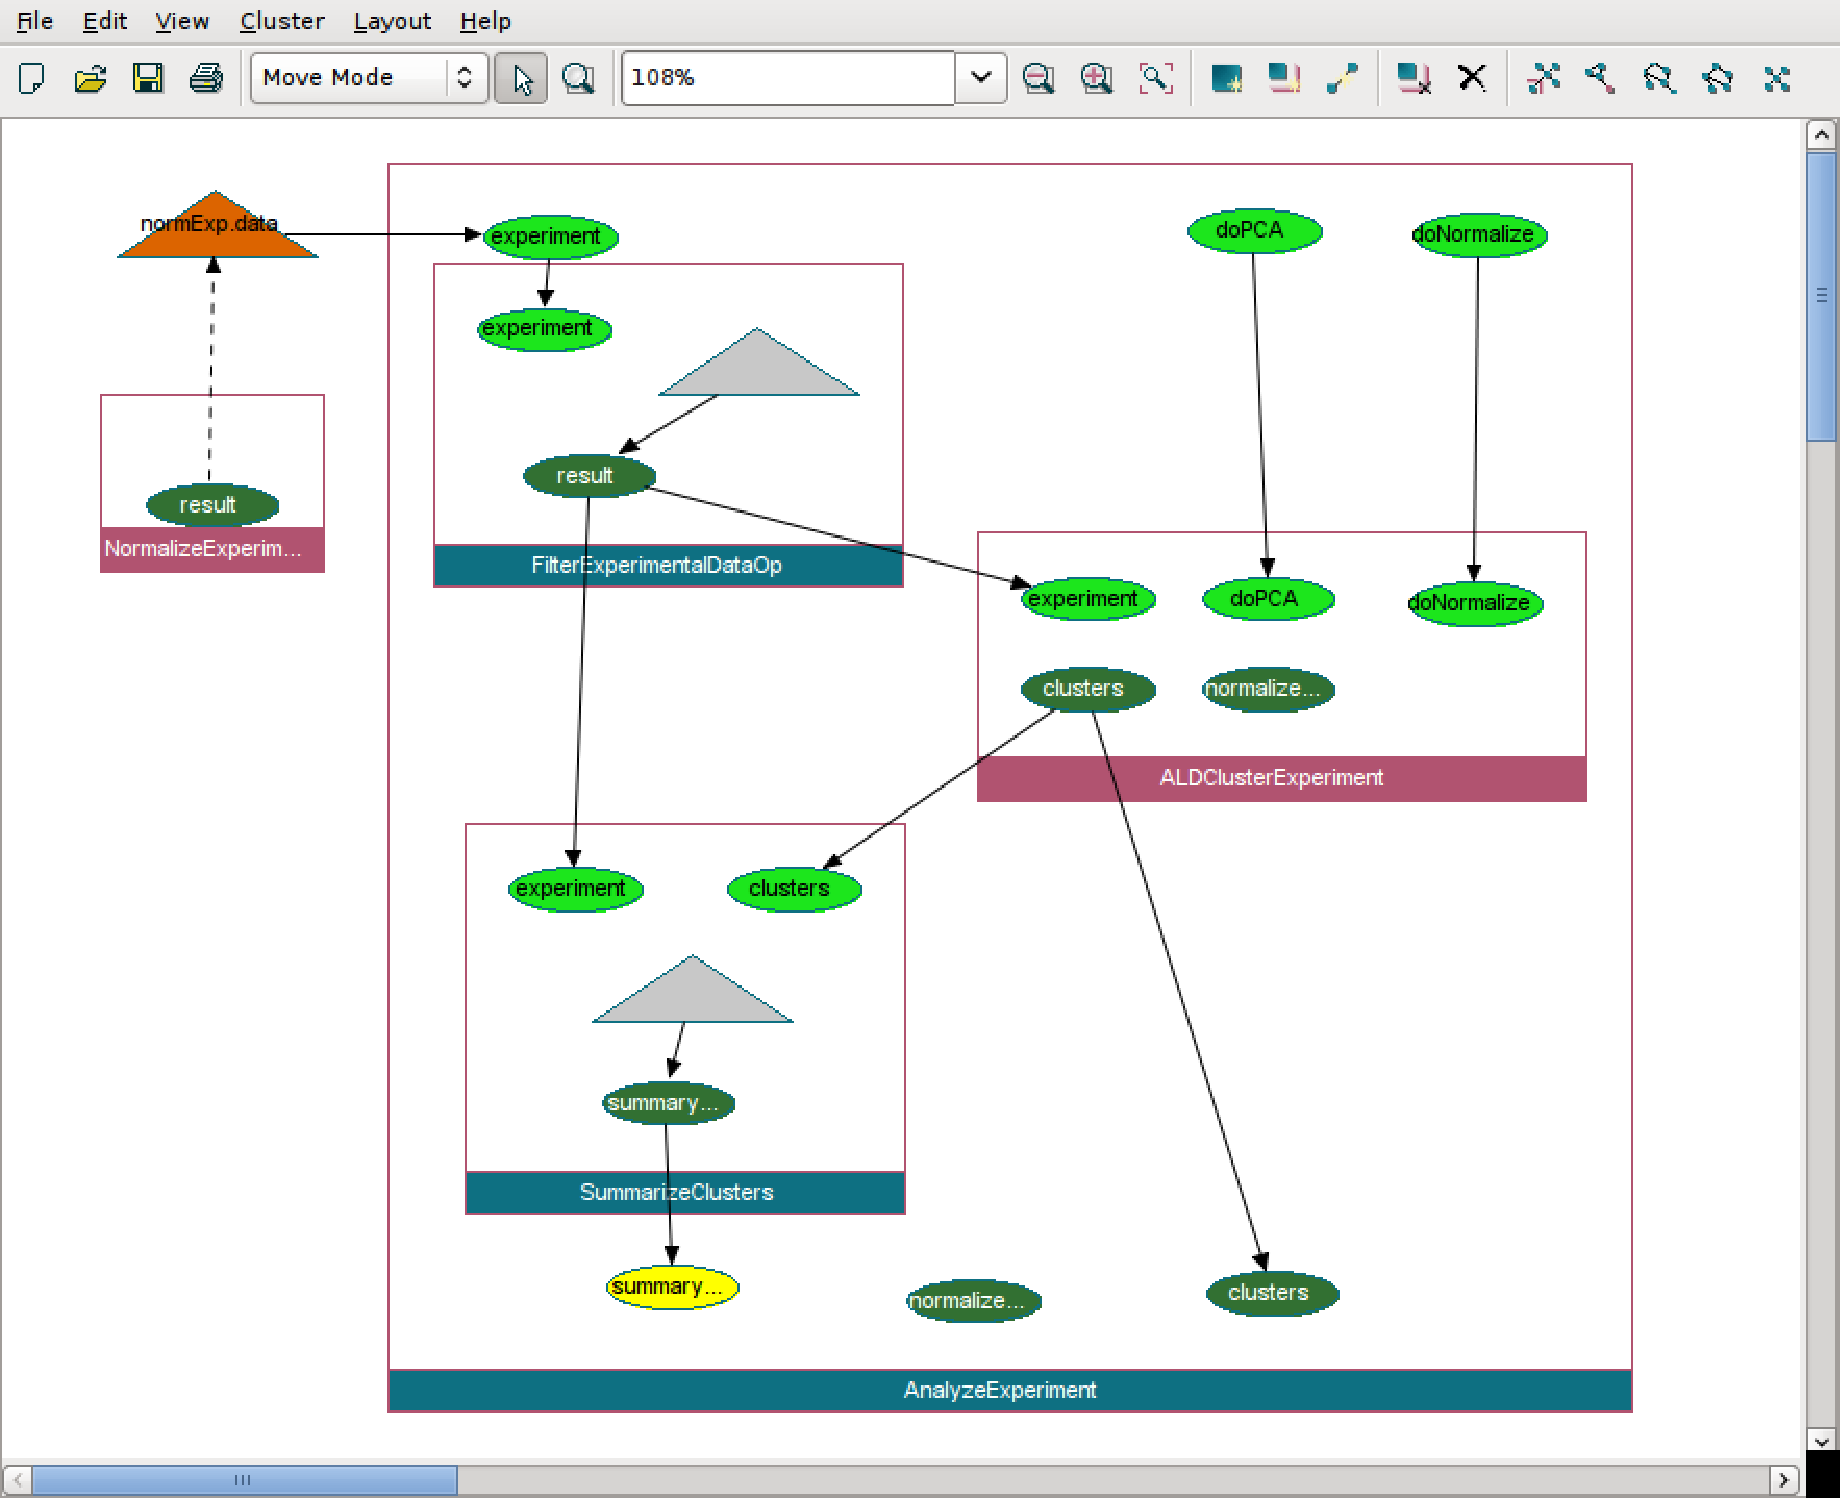
\includegraphics[clip, trim= 10 40 30 70, width=0.9\textwidth]{analyzeData-collapsed-edited}}}
\end{center}
\vspace*{-0.75cm}
\caption[Example of a processing graph.]{\label{fig:DAG2}
A processing graph: the directed acyclic graph represents the application of nested operators. 
Calls to operators are depicted as rectangles, input and output ports as ellipses filled in light or dark green,
respectively. 
The yellow ellipse indicates the result data object
to which this processing graph is linked to.
The triangles relate to newly generated data objects which are colored in grey
unless the data object was read from file.
In this case the triangle is colored orange.}
\end{figure}

The processing graph is stored in XML format in a file accompanying the actual data object file. 
The format basically relies on {\em GraphML}\footnote{GraphML website, 
\href{http://graphml.graphdrawing.org/}{http://graphml.graphdrawing.org/}} with some \alida 
specific extensions. 
If the history is stored externally when a data object is written to disk
depends in general on the data type.
However, when invoking operators from the command line user interface,
most \alida data types will write a history if output of a parameter is
redirected to a file.
\alida uses the
extension \icode{'.ald'} for an {\em \alida\ processing graph} file.
The same is true when reading data.
I.e., in general it depends on the data type if a history is read from file, if
existing. The command line user interface will do this in most cases.

Note, the identity of data is {\em not} preserved in the processing history
across file boundaries. If two (or more) input data for the current top
level operator are loaded
from the same file, both will nevertheless be displayed as different data
nodes in the history. The reason is that object identity is not -- and maybe even cannot -- be checked from the
processing history of former operations.

A processing graph basically consists of operator and data nodes which are connected by edges 
indicating the flow of data, as can be seen from Fig.~\ref{fig:DAG2}. 
The figure shows a screenshot of \mtbc which is a graph visualization tool derived from {\em Chisio}
(see Appendix~\ref{app:chipory} for details).
Within the processing graph each operator node, which is linked to the {\em invocation} of a specific operator,
is depicted as a rectangle with the operator's 
classname in the bottom line.
For each input and output parameter object the operator node features input and output ports which may be conceived as the entry or exit points of data into and out of the operator. These ports are depicted as filled ellipses in light green (input ports) and dark green (output ports),
respectively. Each input port has exactly one incoming edge, while an output
port may be connected to multiple target ports,
depending on where the data is passed to. In Fig.~\ref{fig:DAG2} the result
\icode{'clusters'} produced in the operator \icode{ALDClusterExperiment}
is handed over to the operator \icode{SummarizeClusters} as well as
returned as a result of the operator
\icode{AnalyzeExperiment}. Each port of an operator has an individual name indicating the input or output object associated
with the port. 

In addition to operator nodes and their ports there are also data nodes in the
graph, corresponding to the creation of new data objects, e.g., when data is read from
file, cloned or generated from scratch. These are depicted as triangles filled
in light grey in most cases.
If data is read from file, the triangle is tagged by a string
and colored orange.
%%If the
%%data object extends the class \icode{ALDData} this string gives the name of the file
%%the data was read from. 
If in addition
a processing graph of a
former analysis procedure was read, this history is also included into the
processing graph
and connected by a dashed edge (see top left part of Fig.~\ref{fig:DAG2}).



\subsection{Configuring \alida}
\label{subsec:configure-user}

Sometimes it is desirable to configure 
some properties of \alida or the general behavior of specific operators at
runtime, e.g., to specify initial files or directories where operators should work on. 
\alida basically supports two different ways for user specific configuration:
\begin{itemize}
    \item[a)] environment variables
    \item[b)] properties of the Java virtual machine specified with the \\
    	option \texttt{'-Dproperty=value'} upon invocation of the JVM
\end{itemize}
This order already reflects the priority of the options, i.e., environment
variables overwrite JVM properties.
If for a certain requested property no configuration values are provided by any of these ways,
default settings are used.
Some variables of general interest are used by \alida and are summarized
below.
Further variables may be introduced, e.g., by additional operators implemented in the framework.

In the following list, both the environment variable and the name of the
property are given in the form of \icode{property / environment variable}:
\begin{description}
 \item[\icode{alida.oprunner.level / ALIDA\_OPRUNNER\_LEVEL}] ~

	Used by the graphical operator runner \icode{ALDOpRunnerGUI} and Grappa,
	i.e., the application \icode{ALDGrappaRunner}, to configure which set of
	operators is to be displayed initially in the selection menu.
	Possible options are either all available operators ('standard')             
	or just the ones categorized as being easier to use ('application').
	The default is 'application'.

 \item[\icode{alida.oprunner.favoriteops / ALIDA\_OPRUNNER\_FAVORITEOPS}] ~
	Holds a colon separated list of filenames. Each file
	contains lines of fully qualified operator names which will be unfolded
	in the operator selection window when starting the graphical user interface
	or \grappa (see Sec.~\ref{subsec:userGUI} and~\ref{subsec:grappa}).
	The default is \icode{\$\{user.home\}/.alida/favoriteops}.

 \item[\icode{alida.oprunner.operatorpath / ALIDA\_OPRUNNER\_OPERATORPATH}] ~
	Here a colon separated list of packages may be specified.
	Each package and all its sub-packages 
	are searched for operators in the classpath.
	These operators are incorporated in the tree of available operators
	in the graphical user interface
    and in \grappa.
	This feature is useful to incorporate operators which are not compiled,
	but just added within a jar-archive.
	
 \item[\icode{alida.oprunner.workflowpath / ALIDA\_OPRUNNER\_WORKFLOWPATH}] ~

	Here a colon separated list of directories may be specified each of which
	is searched for workflows saved in a file.
	These workflows are incorporated in the tree of available operators
	in the graphical user interface
        in \grappa.
	The default is \icode{\$\{user.home\}/.alida/workflows}.
	

	
 \item[\icode{alida.versionprovider\_class / ALIDA\_VERSIONPROVIDER\_CLASS}] ~

 Implementation of \icode{de.unihalle.informatik.Alida.ALDVersionProvider} to be used
 for version information retrieval in process documentation
 (Sec.~\ref{subsec:version}).
 
 \item[\icode{alida.version} / --- ] ~
 
 Only available as JVM property, this variable is used by
 \icode{ALDVersionProviderCmdLine} to discover the software version to be stored
 in the history. The class \icode{ALDVersionProviderCmdLine} implements the
 \icode{ALDVersionProvider} interface and gets the version to be used from the
 JVM.
\end{description}



%==================================
\cleardoublepage
\section{The Programmer's View}
\label{sec:programmers}

\subsection{\alida operators}
\label{subsec:operators-programming}

\subsubsection{Using operators}
\label{subsec:using}
To use an operator an object of the operator class needs to be instantiated,
and input data as well as parameters have to be set for this object.
Subsequently, the operator can be invoked using the method
\icode{runOp()}.
After return from that routine the results can be retrieved from the operator.

\textbf{Important note:} Do no invoke an operator directly by its \icode{operate()} method
as this will prevent the processing history from being constructed.
Anyway, this only would be feasible from within the package of the operator
as the abstract method \icode{operate()} is declared \icode{protected}.

An example of how to use an operator is given in Fig.~\ref{exa:useop}.
First, a new instance of the operator is created (line 1), and subsequently
further input parameters are set (lines 2 and 3).
If all required input parameters have been assigned for the operator object,
it can be invoked calling its \icode{runOp()} method (line 4). 
Upon invocation of \icode{runOp()}  the validity of input parameters is checked. 
Validity requires for an operator that all required input parameters
have values different from '\icode{null}'.
In addition, the implementation of an operator may impose further constraints
which, e.g., may restrict the admissible interval of numerical parameters
(see Sec~\ref{subsubsec:implOperators-advanced}).
Subsequent to successful validation, the method 
\icode{operate()}
is invoked. Each operator is supposed to implement this method as it does the
actual work. After return from \icode{runOp()}, the
resulting output data can be retrieved from the operator either directly accessing the member
variables or by getter methods as provided by the specific operator.
Note that the value of the operator parameters may
have changed upon return from \icode{runOp()} due 
to modifications in the \icode{operate()} method.
\icode{runOp()} may throw an exception if validation of inputs and parameters or
data processing itself fails.\\

\begin{figure}[hb]
\lstinputlisting[xrightmargin=.\textwidth,
xleftmargin=.05\textwidth,frame=single]{\demoCodeDir/fixed-snippets/NormalizeExperimentalDataOp-use.snippet}
\caption{\label{exa:useop}An example of how to use an operator, in this case
	\icode{NormalizeExperimentalDataOp}.}
\end{figure}

For the \icode{runOp()} method two version are available.
Besides the one mentioned above without arguments,
the method \icode{runOp(hidingMode)} is available where the value of
\icode{'hidingMode'} influences the visibility of the operator invocation in the
history.
If \icode{'hidingMode'} is \icode{VISIBLE} then the invocation of the operator
is visible in the history.
If the value is \icode{HIDDEN} the invocation of the operator and all is children is hidden.
Finally, if \icode{hidingMode} is set to \icode{HIDE\_CHILDREN} the operator itself is visible,
but all its children are hidden from the history
See Section~\ref{subsec:history} for more details.
\TODO{more explanatiion?, example(s)}

An operator object may be reused to invoke processing
several times as long as input parameters are changed between
subsequent calls of \icode{runOp()}.

\subsubsection{Implementing operators: Basics}
\label{subsubsec:implOperators-basics}

Each operator in \alida is implemented by extending the abstract class \icode{ALDOperator}.
The example given in Fig.~\ref{exa:defineOp}
is the implementation of the demo operator \icode{MatrixSum},
included in the package \icode{de.unihalle.informatik.Alida.demo}.
It
shows
that an operator usually has to be annotated with the \texttt{@ALDAOperator}
annotation provided by \alida.
Some functionality of \alida, most importantly the  execution via automatically generated user interfaces,
 requires this annotation
to register the class as an \alida operator.
If an operator is annotated with \texttt{@ALDAOperator}, a public standard
constructor has to be supplied (see below), otherwise a compilation error will result.
Note that abstract classes can not be annotated with \texttt{@ALDAOperator}.

An operator may declare its preferences for generic execution, i.e., whether to
be or not to be generically executed, by using the parameter
\icode{'genericExecutionMode'} of the annotation. It currently supports four
possible values:
\begin{itemize}\itemseparation{0.1em}
\item \icode{NONE (default)}, to prohibit generic execution completely
\item \icode{SWING}, to allow generic execution via GUI only,
\item \icode{CMDLINE}, to allow generic execution via command line only, and
\item \icode{ALL}, to allow for generic execution in general.
\end{itemize}

Furthermore, operators can be categorized into \icode{'STANDARD'}
or \icode{'APPLICATION'} using the parameter \icode{'level'}.
The latter one is intended to subsume only operators that can easily be applied by non-expert users,
while the first category subsumes all operators. The graphical operator runner included in \alida 
provides two different view modes for either only operators annotated as
\icode{'APPLICATION'}, or all operators registered according to the
\texttt{@ALDAOperator} annotation.

Finally, the annotation also allows to enable batch
processing for an operator. If the parameter \icode{'allowBatchMode'} is set to \icode{'true'},
which is the default, the operator control frame triggered by the GUI operator
runner will show the batch mode tab, and it is expected that the operator
behaves reasonable in that mode. If the parameter is set to
\icode{'false'}, batch mode execution will not be possible at all.

\begin{figure}[h]
\lstinputlisting[xrightmargin=.0\textwidth,
xleftmargin=.05\textwidth,frame=single]{\demoCodeDir/MatrixSum-declare.snippet}
\caption{\label{exa:defineOp}Example deriving the operator \icode{MatrixSum}.}
\end{figure}

There are five issues which have to be taken care of when implementing
an operator, namely
\begin{itemize}\itemseparation{0.1em}
\item	to define the parameters of the operator,
\item	to implement the functionality of operation per se,
\item 	to provide constructors, particularly a public one without arguments
\item	to optionally constrain admissible parameter values,
\item 	and to indicate whether
          this operator prefers a complete processing history
	or a processing history according to data dependencies.
\end{itemize}
The first three issues
are described in the following,
while the last two are deferred to Sec.~\ref{subsubsec:implOperators-advanced}.

\paragraph{Parameters.}
The common way to define the parameters of an operator is by annotation of
corresponding member variables. In addition, since \alida 2.5 it is also possible to
dynamically add and remove parameters via methods provided by \icode{ALDOperator}. For defining
parameters via annotations currently a modified version of the annotation \icode{@Parameter} as under development for ImageJ
2.0$\,$\footnote{ImageJ 2.0 project, \url{http://developer.imagej.net/about}} is used.
The relevant fields of this annotation are listed below and will be detailed in
the following:
\begin{itemize}\itemseparation{0.1em}
\item	\icode{direction} --- direction of the parameter, i.e., \icode{IN},
\icode{INOUT} or \icode{OUT}
\item	\icode{required} --- flag to mark required parameters
\item	\icode{label} --- custom name of parameter
\item	\icode{description} --- short descriptive explanation
\item	\icode{supplemental} --- flag to mark supplemental parameters
\item	\icode{mode} --- importance category of the parameter
\item	\icode{dataIOOrder} --- I/O rank among all parameters of the operator
\item	\icode{callback} --- name of a callback method to be automatically
 invoked upon changes of the parameter's value
%\item	\icode{info} --- parameter is a dummy parameter and exclusively used for
% layout of user interfaces
\item	\icode{modifiesParameterDefinitions} --- changing the parameter's value
 may add or remove parameters of this operator
\end{itemize}

Fig.~\ref{exa:defineParameters} shows an example how parameters are defined this way.
If the \icode{'direction'} of a parameter is set to \icode{'IN'} or
\icode{'INOUT'}, the field \icode{'required'} defines whether this parameter is
required or optional. 
The field \icode{'description'}
of the parameter gives a textual explanation, and the \icode{'label'} may be
used for display purposes.
Setting the field \icode{'supplemental'} to \icode{'true'} declares the
corresponding parameter as supplemental.
Via the Java inheritance mechanism an operator inherits all parameters defined
in its super classes.

\begin{figure}
\lstinputlisting[xrightmargin=.\textwidth,
xleftmargin=.05\textwidth,frame=single]{\demoCodeDir/MatrixSum-parameters.snippet}
\caption{\label{exa:defineParameters}Example defining the parameters of \icode{MatrixSum}.}
\end{figure}

The annotation parameter \icode{'dataIOOrder'} allows to rank parameters
in interface generation. For example, in GUI generation it might be favorable to place the most important 
parameters on top of the window, while parameters of minor importance only
appear at the bottom. Likewise, in command line tools some parameters might be
supposed to appear earlier in the help system than others.
Such a ranking can be achieved by specifying an I/O order. Smaller values refer
to a high importance of the corresponding parameter, larger values to minor importance.
%If a parameter is annotated with \icode{'info'} as \icode{true} the parameter
% is a dummy parameter with no value associated. Rather it is exclusively used to layout automatically
%generated user interfaces. Currently only \icode{'info'} parameters of class
% \icode{String} are supported.

\alida allows to categorize operator parameters according to the level
of knowledge required for their use. Often some parameters of operators are only of interest for experts, and non-expert users
do not even have to be aware of them. To this end each parameter may be
annotated as \icode{'STANDARD'} or \icode{'ADVANCED'}. Accordingly, \alida's graphical user
interface allows to switch the view of parameters between showing only standard parameters and
displaying all.

The annotation parameter \icode{'callback'} allows to specifiy the name of a method of this operator
which is to be automatically invoked by \alida if the annotated parameter's value is changed.
Note the callback method is invoked automatically only when changing the
parameter value using the \icode{setParameter()} method. Callback functions offer amongst others the possibility to
dynamically reconfigure operators depending on the current context. In particular it is possible to
add and remove parameters dynamically. Consider for example an operator allowing for different types
of inputs, e.g.~an \icode{int} or a \icode{float} value. Each of these types requires specific treatment in data
I/O, i.e.~the graphical user interface needs to provide two different graphical elements. Thus,
to handle the different parameters one option would be to add two parameters of the two different
types to the operator and always display both (although only one is needed at a time). Using
callbacks a more elegant way to solve the problem is available. We can add another parameter
\icode{'useRealData'} to the operator which allows to select the type of input
(see Fig.~\ref{exa:callback-define}). If we furthermore
define a callback function for that parameter the user interface of the operator can dynamically be
reconfigured. Depending on the chosen input mode the corresponding input parameter can be added
and the second one be removed dynamically. Adding and removing parameters can be accomplished with
the methods \icode{'addParameter()'} and \icode{'removeParameter()'} of \icode{ALDOperator}.

\begin{figure}[h]
\lstinputlisting[xrightmargin=.0\textwidth,
xleftmargin=.05\textwidth,frame=single]{\demoCodeDir/ALDDynamicOp-parameters.snippet}
\caption{\label{exa:callback-define}Example declaring a parameter which dynamically reconfigures the operator \icode{ALDDynamicOp} in the demo package.}
\end{figure}


Note that changing the set of parameters of an operator
dynamically requires \alida to update its internal representation and also graphical user interfaces
attached to the operator. To this end the programmer is requested to let \alida know that a callback
function changes the parameter set of an operator. This is accomplished using the
annotation parameter \icode{modifiesParameterDefinitions} which is to be set to \icode{MODIFIES\_INTERFACE}.
If changing the parameter value does only modify the values of other parameters,
but not the set of configured parameters,
\icode{modifiesParameterDefinitions}  is to be set to \icode{MODIFIES\_VALUES\_ONLY}.
Note if \icode{modifiesParameterDefinitions} is set incorrectly,
undefined behaviour of the operator may result.
The callback method handling the modification of current parameters known by the operator
should for safety not assume a consistent configuration of the parameters.
For example upon instantiation an inconstitent state my exist temporarily.
Care has been taken to consistently configure the operator in any of the constructors of the operator.

\begin{figure}[h]
\lstinputlisting[xrightmargin=.0\textwidth,
xleftmargin=.05\textwidth,frame=single]{\demoCodeDir/ALDDynamicOp.snippet}
\caption{\label{exa:callback-method}Example of a callback method modifying known parameters of the operator  \icode{ALDDynamicOp} in the demo package.}
\end{figure}

Finally it should be noted that in general care has to be taken when using and implementing callback functions
and reconfiguring the parameter.
For example, mutual calls of different callback functions need to avoid infinite calls.
Consider two parameters \icode{width} and \icode{height} which should adhere to a given aspect ratio.
Thus each of the two parameters is supplied with a callback function which sets the 
other parameter according to the new value and the aspect ratio.
If this is however done via the \icode{setParamteter()} method this will provoke infinite recursion.
To avoid this either the parameter can be changed using directly assigning a value,
or -- probably the better choice -- using \icode{setParamteter()}  only in case that the value indeed needs to be set to a new value.
Otherwise, if old and new values are identical, nothing is to be done.

\paragraph{Operator functionality.}
The method \icode{operate()} implements the functionality of the operator. All data
passed into and returned from the operator have to be passed through the parameters of the operator.
They may be set and retrieved with the generic
\icode{getParameter(name)} and \icode{setParameter(name,value)} methods
of \icode{ALDOperator}, by specific setter- and getter-methods as provided by
each operator, or by
directly accessing the member fields if allowed.
To invoke the processing within an operator, i.e., to run its \icode{operate()}
routine, the final method \icode{runOp()} supplied by \icode{ALDOperator} needs to be called by the user of an operator.

\paragraph{Constructors.}
As noted above, 
for automatic code generation and documentation capabilities as well as generic execution 
of an operator,
the operator class needs to implement 
a public standard constructor 
as shown in Fig.~\ref{exa:constructor}.
This is, however, not necessary if the operator is only to be used explicitly
by the programmer and is not annotated.
Further convenience constructors may be implemented which additionally set
parameters.

\begin{figure}
\lstinputlisting[xrightmargin=.\textwidth,
xleftmargin=.05\textwidth,frame=single]{\demoCodeDir/MatrixSum-constructor.snippet}
\caption{\label{exa:constructor}Constructors of \icode{MatrixSum}.}
\end{figure}

\paragraph{Processing history.}
As decribed in Sec~\ref{subsec:using} the visibility of an operator invocation in the
processing history may be
influcenced by the parameters of the  \icode{runOp()} method.
By this means the visibility of each operator invocation may be set to
\icode{VISIBLE}, \icode{HIDDEN}, or \icode{HIDE\_CHILDREN}.
This also allows to determine the visibility of further operators directly
invoked by their \icode{runOp()} method but not of operators indirectly invoked.
Thus, the implementor of an operator may influence the visibility
of its own invocation using the method \icode{setHidingMode(hidingMode)}.
The main usage of this method is to set the operators visibility to \icode{HIDE\_CHILDREN}
to hide recursive calls to further operators from the history.
This also hides operator calls which are indirectly invoked arbitrary methods used when implementing
the \icode{operate()} method.

\textbf{Important note:} It is strongly recommended that an operator
does not rely on specific initializations, e.g., of private fields, that are
performed in a constructor (besides the default constructor)
and depend on the values of input parameters. Rather,
it is advised that upon invocation of the \texttt{operate()} method an operator performs all necessary initializations according to the parameter settings.
This allows to take into account changes of parameter values subsequent to
construction of the operator object by using the \texttt{setParameter(\ldots)}
method or dedicated setter methods.
Otherwise generic execution of the operator is not feasible and
the operator should not be released for generic execution.

\begin{figure}[tb]
\lstinputlisting[xrightmargin=.\textwidth,
xleftmargin=.05\textwidth,frame=single]{\demoCodeDir/ApplyToMatrix-parameters.snippet}
\caption{\label{exa:operatorAsParameter}An example of an operator as a parameter in the operator \icode{ApplyToMatrix}}
\end{figure}

\subsubsection{Implementing operators: Advanced techniques}
\label{subsubsec:implOperators-advanced}

\paragraph{Operators as parameters.}
\alida supports as parameters of an operator also any (other) \alida operator.
This is shown for the demo operator \icode{ApplyToMatrix} in Fig.~\ref{exa:operatorAsParameter}.
In this case, the class \icode{ALDSummarizeArrayOp} is an abstract operator 
which takes a 1D array as input and returns a summarizing scalar.
Now, one may implement concrete examples of such a summarizing operation. 
As examples \alida ships with operators implementing
the summation (\icode{ALDArraySum}), mean (\icode{ALDArrayMean}) and minimum
(\icode{ALDArrayMin}) operations.
Each operator implements the  \icode{operate()} method and has to supply a
standard constructor.
As shown in Fig.~\ref{exa:ALDArraySum},
the  operator \icode{ALDArraySum} is declared as operator on the
\icode{'STANDARD'} in contrast to \icode{'APPLICATION'} level, as
it is not expected to be invoked as an application.
However, setting the level to standard in the menu of the graphical user interface
stills allows their direct execution.
When extending the super class \icode{ALDSummarizeArrayOp}, it is necessary to
annotate the class with \icode{@ALDDerivedClass} in order to allow \alida's data
I/O mechanisms to find the derived class in automatically generated user
interfaces.
This holds for other parameter types as well, see Sec.~\ref{subsubsec:datatypes}.

\begin{figure}
\vspace{4mm}
\lstinputlisting[xrightmargin=.\textwidth,
xleftmargin=.05\textwidth,frame=single]{\demoCodeDir/ALDArraySum-constructor.snippet}
\caption{\label{exa:ALDArraySum}The operator \icode{ALDArraySum} as an operator in standard level.}
\end{figure}

\paragraph{Constraints on admissible parameter values.}

The implementation of an operator may impose 
custom constraints on the input parameters
beyond the general requirement, that all required input parameters
need to have non-null values.
This is achieved by overriding the method \\
\begin{lstlisting}[xrightmargin=.00\textwidth, xleftmargin=.0\textwidth,frame=single,numbers=none]
  public void validateCustom() throws ALDOperatorException
\end{lstlisting}
which, e.g., may restrict the admissible interval of numerical parameters.
This method is called by \icode{runOp()} prior to the invocation of the
\icode{operate()} method of an operator. It is supposed to throw an exception
of type \icode{ALDOperatorException} with type \icode{VALIDATION\_FAILED} and
a striking error message if the validation was not successful.

\paragraph{Preference for history graph construction.}
Each operator may specify a preferred
way to create the processing history by setting
its member variable \icode{'completeDAG'}.
The default mode is a complete processing history,
i.e., \texttt{completeDAG == true}. This works in all cases,
but potentially includes additional operator invocations as performed in the
\icode{operate()} method which do not directly influence
the values of the object for which the history is constructed.
To generate a leaner history graph the programmer of an operator
may choose to set \icode{'completeDAG'} to \icode{false}, see
Section~\ref{subsec:history} for details.

In case an implementor decides to completely disable the construction of the processing history 
this can be accomplished with the static method \icode{setConstructionMode()} of
the \icode{ALDOperator} class.


\paragraph{Progress events.} \alida provides a mechanism for operators
to send status and progress messages to the user during execution. These messages
are shown in the status bar of the operator control windows
(Sec.~\ref{subsubsec:controlWin}) and also in Grappa's log panel
(Sec.~\ref{subsec:grappa}). Accordingly, in constrast to output to standard out,
which is not guaranteed to reach the user, these messages will always be visible
to the user. For triggering such messages, an operator has to fire an event of
type \icode{ALDOperatorExecutionProgressEvent} using the method\\
\begin{lstlisting}[xrightmargin=.00\textwidth, xleftmargin=.0\textwidth,frame=single,numbers=none]
  protected void
	  fireOperatorExecutionProgressEvent(ALDOperatorExecutionProgressEvent ev)
\end{lstlisting}
The event takes a message string as argument during construction which is then
displayed to the user.

\subsubsection{Implementing operators: Parameters}
\label{subsubsec:datatypes}

\paragraph{Derived classes.}
As noted above, 
if an instance of a class is to be supplied in an automatically
generated user interface as a value for a parameter of one of its super classes,
\alida requires the annotation \icode{@ALDDerivedClass}.

\paragraph{Parameterized classes.}
\alida provides automatic I/O of primitive data types, enumerations, arrays, collections,
and operators.
In addition, so called \textit{parameterized classes} are supported.
Any Java class may be declared to be a parameterized class in \alida
by annotating the class with \icode{@ALDParametrizedClass} as shown for the
class \icode{ExperimentalData1D} in Fig.\ref{exa:parametrizedClass}.
The class is annotated by \icode{@ALDParametrizedClass},
and all members to be configured via \alida's user interfaces are
to be annotated with \icode{@ALDClassParameter}. This annotation offers the
following arguments:
\begin{itemize}
  \item \icode{'label'} --- name of the parameter, field has same
	semantics as for parameters of operators
  \item \icode{'dataIOOrder'} --- I/O rank of the parameter	 
  \item \icode{'mode'} ---
	importance of the parameter, i.e., \icode{'STANDARD'} or \icode{'ADVANCED'}	 
  \item \icode{'changeValueHook'} --- post-processing routine after reload (see
  below)
\end{itemize}

The first three annotations share their semantics with their counterparts in the
\icode{@Parameter} annotation of operators
(cf.~Sec.\ref{subsubsec:implOperators-basics}).
Only the forth one is special to parameterized classes. On loading or saving
operator configurations, i.e.~the values of its parameters, also objects of
parameterized classes used as parameters have to be handled. To this end these
are also converted to XML format. However, in doing so only {\em annotated}
member variables of the parametrized class are taken into account. Consequently,
also only these member variables of the object will get proper values after
reload.
In some cases, however, this might lead to inconsistencies in an object's state
after reload. Consider for example a parameterized class representing a set of
points. Most likely this class will define a member variable of a list type
which holds the points, and as this member holds the core data of the data
type, it will be annotated.
Now, for efficiency of implementation it might be of advantage to define another
member variable keeping track of the number of points in the list, usually not
being annotated. To ensure that this variable is also correctly set on reload of
the object, the \icode{'changeValueHook'} argument can be used. It expects a
string defining a method of the class at hand which is to be called after all
annotated member variables have been properly set during reload. The method may
then perform some kind of post-processing of the object's configuration, i.e.,
set the point counter variable to the number of points found in the given list.
Note that the hook method may not expect any arguments.

The above annotations are
the only implementational overhead to allow \alida to automatically generate user interfaces where the parameterized class acts as a parameter.
Operators acting as parameters of other operators may be viewed as
special cases of parameterized classes.


\begin{figure}
\lstinputlisting[xrightmargin=.\textwidth,
xleftmargin=.05\textwidth,frame=single]{\demoCodeDir/ExperimentalData1D.snippet}
\caption{\label{exa:parametrizedClass}The class \icode{ExperimentalData1D} as an example of a parameterized class.}
\end{figure}

\paragraph{Automatic documentation}

The value of each \icode{'IN'} and \icode{'INOUT'} parameter is recorded
upon invocation of an operator via its \icode{runOp()} method using the method \icode{toString()}
of the parameter class for later storage in the processing history.
Thus, it is recommended to supply an appropriate \icode{toString()}
method for data types used as parameters to yield informative histories.

If a parameter of an operator is expected to be documented in the data flow of
the processing history, it
may be of any Java class being uniquely
identifiable. This excludes only primitive data types, interned strings
and cached numerical objects.
If the parameter need not to be part of the data flow, all classes are
acceptable.

Note that before returning from \icode{runOp()}, additional documentation is
done for output objects derived from the abstract class \texttt{ALDData}.
This class essentially features a property list which may 
be used to augment data objects, e.g., by a filename or URL specifying 
the origin of the data.

\subsection{Data I/O provider}
For the generic execution of operators via command line or graphical user
interfaces in \alida, knowledge is required about how to perform input and
output operations for parameter data objects.
In particular, in graphical contexts \alida requires functionality to query 
values for parameter objects from the user via graphical input components, and
to adequately visualize parameter values graphically. For invocation of operators from 
command line, parameter data objects need to be instantiated from textual input,
and parameter objects need to be transformed into a user-friendly textural representation. 

To enable flexible data I/O \alida implements an easily extendable provider mechanism. 
A {\em provider} is a class implementing the functionality to perform I/O for
objects of specific data types, i.e., to instantiate objects from given user
input and visualize their values graphically or in a textural fashion. These
providers are managed by {\em data I/O managers} which keep track of available
providers and provide methods for getting provider objects for specific data
types at run-time, e.g., to facilitate the automatic generation of graphical user interfaces.

Currently, two user interface contexts are implemented in \alida, i.e., a tool
for executing operators from command line (cf.~Sec.~\ref{subsec:userCmdline})
and a graphical operator runner based on Java Swing (cf.~Sec.~\ref{subsec:userGUI}). For both contexts \alida already offers 
built-in providers for a large variety of different parameter data types. In detail, all primitive 
data types available in Java (e.g., int, double, boolean) as well as corresponding wrapper data 
types (e.g., Integer, Double, Boolean), enumerations, arrays of primitive and wrapper data types, 
and also all kinds of Java collections\footnote{The only exception are
collections of collections which are not yet supported.} are supported
out-of-the-box.
Also, operators may be used as input parameters of other operators, and by the concept 
of parameterized classes (Sec.~\ref{subsubsec:datatypes}) \alida allows for easy extensibility. In some cases,
however, it might be necessary to implement a data I/O provider for a certain 
parameter data type from scratch. 
Below we outline the basics of how to accomplish this.
 
All providers in \alida are registered by I/O managers upon start-up. These managers basically
keep a map of data types and related providers and allow the framework to get a provider object
for a certain parameter data type at run-time. 
Additionally, they may give hints to the provider classes to adapt their
functionality to the current mode of operation.
The type of these hints is specific to the context, e.g., command line or GUI,
and will be described below.

To enable the managers to automatically register 
all provider classes available on the classpath, it is necessary to annotate the
provider classes with the \alida annotation \icode{@ALDDataIOProvider}. 
This annotation features the field \icode{'priority'} which is used to
select a provider in case that several providers handle the same data type.
This allows, e.g., to override providers delivered by \alida with custom made providers.
In addition, all providers have to 
implement the interface 
\vspace*{0.5cm}
\begin{code}
	de.unihalle.informatik.Alida.dataio.provider.ALDDataIO 
\end{code}

\vspace*{-0.25cm}
It basically defines a single method that all providers need to implement:
\vspace*{0.5cm}
\begin{code}
	public Collection<Class<?>> providedClasses();
\end{code}

\vspace*{-0.25cm}
This method is used by the I/O managers upon start-up to gather information about
which classes a specific provider supports, i.e., to fill its maps. Of course,
apart from this method the actual functionality of a provider class depends on the user interface 
context in which it is to be used. In the following subsections we will now describe the specifics
of implementing providers for the Java Swing (Sec.~\ref{subsubsec:implProviderSwing}) and 
the command line context (Sec.~\ref{subsubsec:implProviderCmdline}).
  
\subsubsection{Implementing a Swing data I/O provider}
\label{subsubsec:implProviderSwing}
To enforce all providers dedicated to the Swing context to implement the corresponding graphical 
data I/O concept, \alida defines a specific interface for the Swing context: 
\vspace*{0.5cm}
\begin{code}
	de.unihalle.informatik.Alida.dataio.provider.ALDDataIOSwing 
\end{code}

\vspace*{-0.25cm}
This interface subsumes all methods to be implemented by Swing providers.

\paragraph{Graphical data input.} The basic workflow which
\alida defines for graphical input of a parameter data object is as follows. First a graphical 
component needs to be generated by the provider suitable for querying values 
from the user. Such a component is for example given by a checkbox to query the user for a boolean 
value, a textfield to query for a string or number, or a combobox to let the user select a single
or multiple values from a larger collection. This component is then included in graphical user
interfaces, e.g., the graphical control windows of \alida's graphical operator runner.
Subsequently, once the user has entered appropriate values, functionality is required 
to read the specified values from the graphical component. 

Accordingly, the interface basically defines the following two methods:
\vspace*{0.5cm}
\begin{code}
  public abstract ALDSwingComponent createGUIElement(
      Field field, Class<?> cl, Object obj, ALDParameterDescriptor descr);

  public abstract Object readData(
      Field field, Class<?> cl, ALDSwingComponent guiElement);
\end{code}

\vspace*{-0.25cm}
The first method is supposed to return a graphical component suitable for being included in 
graphical control windows. In general, \alida does not define any strict rules
for these components except that they have to be of type
\icode{ALDSwingComponent} and implement the methods defined in that interface.
Objects of this type basically wrap an object of type \icode{JComponent}. 
Only the latter one is actually included in the configuration and control windows. 
Although there are principally no restrictions on the 
design of the components returned by providers, note that proper automatic GUI
layout is only possible if the different 
components do not vary too much in their sizes. Hence, it is advisable to layout the components 
in such a way that they only fill one row in a panel. Elements which naturally obey to this rule 
are for example buttons, text fields, and combo- or checkboxes. If you require more complex 
components to query values from the user, one solution could be to return a button as main GUI
component by which a new window can be opened with an arbitrary size where the actual parameter 
values can then be entered. 
This technique is employed, e.g., by \alida's standard providers for
parameterized classes and collections.

Besides wrapping a graphical component, objects of type
\icode{ALDSwingComponent} have to implement an event reporter interface. This
interface lays the foundation for \alida to be able to visualize the current state of an operator's configuration in its control windows in real-time. The interface
basically enforces the graphical component to trigger events on changes of the values specified
in the graphical component. For most providers relying on Swing components as graphical components
it is sufficient to implement listeners for the Swing components and simply forward Swing events
as \alida events of type \icode{ALDSwingValueChangeEvent} to the framework.
Refer to the API documentation of
\icode{de.unihalle.informatik.Alida.dataio.provider.swing.components.ALDSwingComponent}
and related event reporter and handler classes in the package
\icode{dataio.provider.swing.events} for more details. Also note that
\alida already provides implementations of graphical elements for data
I/O of common data which subclass \icode{ALDSwingComponent}. They are to be
found in the package \icode{dataio.provider.swing.components} and can be used
out-of-the-box.

The method \icode{createGUIElement(field, cl, obj, descr)} takes four
arguments as input.
The argument \icode{'cl'} specifies the class of the parameter object which 
should be read by the component (which is of special interest for providers supporting various
data types), while the \icode{'obj'} argument allows to pass a default value to
the provider. The argument \icode{'descr'} allows to hand over additional
information to the provider about the operator parameter with which the object is associated. \alida uses this information, e.g., for 
generating more meaningful labels in the graphical control windows. Note that if no descriptor is
available, \icode{'null'} is also a valid value, hence, providers must account
for this specical case.
The first argument \icode{'field'} can be ignored by most
providers. There are only a few providers where the object class is not sufficient 
to instantiate a parameter object, and where in addition the field associated
with the member variable representing the parameter is required to have all relevant information available. 
One example are collections in Java, where the data type of the
elements contained in the collection is not obvious from the class of the collection itself.

The second method \icode{readData(\ldots)} of the \icode{ALDDataIOSwing} interface takes as argument a 
formerly generated graphical
component \icode{'guiElement'} and is supposed to return an object of the
specified class. The object should
contain the value as currently specified by the graphical component.
The \icode{'field'} argument can most of the time be ignored by the provider,
refer to the previous paragraph for details. 

In addition to the formerly discussed methods the interface defines a third method
\vspace*{0.5cm}
\begin{code}
  public abstract void setValue(
      Field field, Class<?> cl, ALDSwingComponent guiElement, Object value);
\end{code}

\vspace*{-0.25cm}
which is supposed to set new values in the graphical component. Its arguments are quite similar 
to the \icode{createGUIElement(\ldots)} method. The new value to be set is
specified by the \icode{'value'} argument.

\paragraph{Graphical data output.} For performing graphical data output the
Swing provider interface defines the method
\vspace*{0.5cm}
\begin{code}
  public abstract JComponent writeData(Object obj, ALDParameterDescriptor d);
\end{code}

\vspace*{-0.25cm}
It basically takes an object \icode{'obj'} as input and generates a suitable
Java Swing component to properly visualize the object's value. Note that the class of the object is directly derived from 
the object itself. The additional descriptor argument is used to enhance the graphical component
with more information about the object. The object might be \icode{'null'},
i.e., the provider has to check its value prior to accessing the object
directly. For components generated by this method the same rules hold as for the graphical input components. In particular, ensure that each component does not exceed the height of one row in a panel to enable proper GUI layout.

\paragraph{Interaction level.} 
The I/O manager for the Swing context gives providers a hint on the amount of
user interaction level the providers should generate.
The reason is that 
there are situations when only warnings should be signaled to the user or no
pop up of windows and user interaction is intended at all. To request the
desired level of interaction and to modify the setting, the Swing data I/O
manager offers the following methods:
\vspace*{0.5cm}
\begin{code}
 public ProviderInteractionLevel getProviderInteractionLevel()

 public void setProviderInteractionLevel(ProviderInteractionLevel level)
\end{code}

\subsubsection{Command line provider}
\label{subsubsec:implProviderCmdline}

In analogy to Swing providers each command line provider is required to
implement 
\vspace*{0.5cm}
\begin{code}
	de.unihalle.informatik.Alida.dataio.provider.ALDDataIOCmdline
\end{code}

\vspace*{-0.25cm}	
This interface defines two methods to be implemented, namely
\vspace*{0.5cm}
\begin{code}
  public abstract Object readData(Field field, Class<?> cl, String valueString);

  public abstract String writeData(Object obj, String locationString);
\end{code}

\vspace*{-0.25cm}
The first method is expected to instantiate an object of class \icode{'cl'} from
the string \icode{'valueString'}.
For the meaning of the argument \icode{'field'} see the subsection
on Swing providers.
In general, the syntax of the value string depends on the data type
and may freely be defined  by the implementation of the provider.
However, \alida offers the notion of a standardized command line provider
taking care of derived classes as  well as reading and writing to and from files
(see below).
Additionally, \alida provides a command line provider for parameterized classes
featuring a specific syntax (see Sec.~\ref{subsubsec:datatypes}).  
If appropriate, it may be sensible to adopt the syntax for other
providers as well.

The method \icode{writeData(\ldots)} is used to format the given object to textual
form into a string.
The \icode{'locationString'} specifies whether this textual representation is
to be returned as the result of the method or should be written to, e.g., a
file.
In the latter case the string returned may contain information of this process,
e.g., return a note that the object was written to a specific file.
As for the syntax of  the \icode{'valueString'} in \icode{readData(\ldots)}, the
syntax of the  \icode{'locationString'}  may in principle be freely defined by each
provider.
However, it is advisable to adhere to \alida's standard definitions by the
standardized command line provider as described in
Sec.~\ref{subsec:userCmdline}.
In addition, the \icode{'locationString'} may also be used by a provider as
a format string to modify the textual representation of the object generated.


\alida features a so called {\em standardized commandline provider}
to generically handle data I/O from and to file, and for the input of derived
classes, in the abstract class \icode{ALDStandardizedDataIOCmdline}.
It is easy to implement new providers extending this class and,
thus, to automatically inherit the ability to handle file I/O and derived
classes.
It is only required to implement the two abstract methods
\vspace*{0.5cm}
\begin{code}
  abstract public Object parse( Field field, Class<?> cl, String valueString);

  abstract public String formatAsString( Object obj);
\end{code}

\vspace*{-0.25cm}
of \icode{ALDStandardizedDataIOCmdline}.

The first method should instantiate an object of class \icode{'cl'} from
the \icode{'valueString'} quite similar to the method \icode{readData(\ldots)}
introduced above, however, making no prior interpretation regarding a file to
use or derived class to return.
This has already been handled by the class \icode{ALDStandardizedDataIOCmdline}
prior to calling \icode{parse(\ldots)}.
Likewise, the method \icode{formatAsString(\ldots)} should always return a textual
representation of the given object as return value.
If it is necessary to use formatting information provided as part of
the argument \icode{'locationString'} of \icode{writeData(\ldots)}, the method
\vspace*{0.5cm}
\begin{code}
  public String formatAsString( Object obj, String formatString)
\end{code}

\vspace*{-0.25cm}
may be overridden.

As mentioned, I/O managers may give providers hints to adapt their
functionality.
In the case of the command line context this is the request to
read or write a history file in case the I/O is to be performed from or
to file.
The method \icode{isDoHistory()} may be used to inspect the state of the manager.
The standardized command line provider adheres to this standard.

\subsection{XML provider for external representation}

XML providers are used to store and retrieve parameter configurations of
operators and workflows.
As a consequence, (typically) transient data are not stored (and retrieved).

\icode{ALDXMLObjectType} is the base type of all Alida XML data types.
In only contains the classname (fully qualified classname).
Extending types will add the data itself.
Such XML representations do not only contain the data itself,
but allow to infer the class of the represented object. 
Thus, it is feasible to instantiate the correct object and fill it with all
data as stored in the XML object.

Currently there exist the following extending types:

\begin{tabular}{l|l}
\icode{ALDXMLArrayType} & to hold 1D arrays and collections \\
\icode{ALDXMLParametrizedType} & for parametrized classes holding a list of
(key,value)-pairs,\\
& where the values are of type \icode{ALDXMLObjectType} \\
\icode{ALDXMLEnumType} & for an enum value, which is just represented by a string \\
\icode{ALDXMLAnyType} & to hold any type, used, e.g., for primitive data
types,\\ & numerical data types
\end{tabular}

For writing an XML provider on your own
\begin{enumerate}
\item	create an XML beans object which can hold the data item.
	This may be a native XML beans data type like \icode{XmlInt} or
	\icode{XmlString}, or a custom XML beans data type typically created via an
	XML schema and the XML bean compiler (\icode{xmlbean} ant task).
\item	create an object of type \icode{ALDXMLAnyType},
	\begin{itemize}
	\item	set its member \icode{'className'} to the class name of the data item
	\item	set its value to the XML beams object created in step 1.
	\end{itemize}
\end{enumerate}

\subsection{Automatic data type conversion}
\label{subsec:converter}

\alida features a generic mechanism for data type conversion.
This conversion mechanism is currently used within the graphical workflow editor \grappa
(see Sec.~\ref{subsec:grappa}).
\grappa allows to connect an output port of one operator to the input port of another operator
if the data types of the underlying parameters are compatible.
The data types are defined as compatible if either the target data type is
assignable from the source data type according to the Java class hierarchy or
an appropriate data type converter is supplied.
For example \alida ships with the converter 
\icode{ALDNumberConverter} between numeric data types, obviously
with potential loss of precision.
Likewise conversion from vectors to 1D arrays is supported
by the class \icode{ALDVectorNativeArrayConverter}.

Similar to data I/O providers, data type converters are registered on start-up by 
a singleton instance of the class \icode{ALDDataConverterManager}.
This manager redirects conversion requests to appropriate
converters.
This requires each data type converter to implement the interface
%%\vspace*{0.5cm}
\begin{code}
de.unihalle.informatik.Alida.dataconverter.ALDDataConverter
\end{code}
and to be annotated with the \alida annotation
\icode{@ALDDataConverterProvider}.
In analogy to \alida's data I/O provider a priority may be specified which is used
by the converter manager to resolve competion between multiple converters for a
given pair of data types to be converted.

A data type converter has to implement the methods
%%\vspace*{0.5cm}
\begin{code}
Collection<ALDDataConverterManager.ALDSourceTargetClassPair> providedClasses()
boolean supportConversion(Class<?> sourceClass, Type[] sourceTypes, 
                               Class<?> targetClass, Type[] targetTypes)
\end{code}
The first one is called upon start-up and it has to return pairs of source and
target data types which the converter is able to handle.
However for parameterized types this only indicates that the converter can in principle handle conversion 
for these classes but depending on the type parameters still may refuse to do so.
The second method, \icode{supportConversion} states precisely if conversion is supported
taking also type parameters passed as arguments into account.

The actual conversion is performed invoking the method
\begin{code}
Object convert(Object sourceObject, Type[] sourceTypes,
               Class<?> targetClass, Type[] targetTypes)
\end{code}
As stated above this method is typically not invoked directly but via the 
\icode{ALDDataConverterManager}.

Note that both converters supplied by \alida are implemented as an \icode{ALDOpertor}.
Thus the conversions are reflected within the processing history unless
they are intentionally hidden (see Sec.~\ref{subsec:operators-programming} and \ref{subsec:history}).

\subsection{The processing history}
\label{subsec:history}

Data processing pipelines in \alida build on the idea of operators that
manipulate data objects. According to the specification of \alida operators
(see Sec.~\ref{subsec:operators-user}), data objects that are to be manipulated by a
certain operator will have to be stored in member variables of the
operator annotated as operator parameters with direction '\icode{IN}' or '\icode{INOUT}'.
Result data objects of an operator will be stored in member
variables annotated as parameters with direction '\icode{OUT}' from where the user of
the operator can access the result object for further processing tasks.

Logging the complete processing history of individual objects enforces \alida
to link data objects used as inputs or resulting as outputs from operator
invocations directly to the manipulating operators. These links essentially form the
base to lateron build the history graph representation for each object ever
seen by any of the \alida operators during a processing chain.

\subsubsection{Basics of the history concept}
\label{subsubsec:basicshistory}
The key for logging all operator invocations and the corresponding operator
configurations during each run of a processing pipeline is \alida's
port hash. Within this hash all objects participating in the
processing pipeline are registered. 
For each object a link to the relevant port of the most recent operator
invocation, which manipulated or generated the object, is stored
as a reference to a port object in a weak hash map. This kind of
hash map only holds \textit{weak} references to objects, which allows the Java virtual machine
to destroy the objects if they are not referenced somewhere else anymore. The
port hashmap allows to link input and output ports of operators as well as data
ports according to the data flow, and to lateron traceback the sequence of
manipulations for each object manipulated during the course of the processing.

The complete history of a data processing chain is only implicitly represented
by the links between the different kinds of ports. Each operator invocation is
represented by an object of type \icode{ALDOpNode} which consequently needs to
store its current inputs and outputs. The \icode{ALDOpNode} class defines input
and output ports for input and output objects of an operator. 
Data ports represent newly created data objects that were not passed to an
operator as input so far. Such objects appear, e.g., when a new data object is
allocated to store the results of an operator. Altogether these ports provide
the functionality to establish connections between new data and inputs and
outputs of operators. 

The history of a data object is built on
request traversing the connections that are stored in \alida's port hash. While
many different objects can be linked to a single processing chain, i.e.~can be
manipulated by operators during one run of various operators, a single object
has always its own individual manipulation history. This history is given by a
certain path within the manipulation graph of the complete processing chain. 
The starting point of the object's path is always the most recent operator
invocation which involved manipulations of the object. Consequently, the link to
the port associated with this operator invocation is the one stored in the port hash.
Tracing back the history from this port then allows to recover all object
manipulations and build up the final history graph. Neither the programmer nor
the user of an operator have to take care of the data stored in the port hash or
the correct logging of operator invocations. Object registration and the update of
port links are done automatically each time an object is fed into an operator or
taken out of an operator as result. In particular, the \icode{runOp()} method of
\icode{ALDOperator} takes care of all this and handles the history data management
internally. 

The only situation when programmers get in touch with the processing history and the port
hash is when the processing history of an object is to be created explicitly,
e.g., to be saved to disk. While this
is done automatically for some \alida data types which provide read and write
methods, there is still the need for programmers to take care of
this for own data types not providing appropriate read and write routines so far.

\subsubsection{Accessing history data}
At any point in time during data processing the processing history of
any object manipulated is implicitly represented in the processing history graph. 
To access this data and transfer the processing
history from the implicit to an explicit representation, it is possible to 
generate this history using the static method
\icode{createGraphmlDocument()} of the class \icode{ALDProcessingDAG}.
This creates the processing history associated with the object
in a graph data structure as generated by
\href{http://xmlbeans.apache.org/}{\em XmlBeans}
\footnote{\url{http://xmlbeans.apache.org/}}. It is based on the XML schema definition of
\href{http://graphml.graphdrawing.org/}{\em GraphML}
\footnote{\url{http://graphml.graphdrawing.org/}} with \alida
specific extensions. Although intended for writing and reading the history to or from file (see next paragraph) in the first place, this data structure may also be used to inspect the processing graph as constructed directly from Java.

%Although all data about the processing history is stored in XML format, and
%although the data could principally be extracted from the database directly as
%XML tree, \alida currently only supports the saving to file. 
%The main reason for
%this is that graph visualization of the processing history is the most intuitive
%way to explore such kinds of hierarchically structured data. While direct
%analysis of the XML data might in principal allow for automatic history
%analysis such a scenario will most probably rarely occur in practice.

%The port hash providing the entry ports into the implicit processing history graph is implemented in
%class \icode{ALDPortHash}. As this class is completely invisible from outside of the \icode{de.unihalle.informatik.Alida.operator}
%package 
To store the processing history in XML format, to be more precisely in
{\em GraphML} format, the class \icode{ALDOperator}
provides a static method to save the processing history of
an object to an XML file:
\begin{code}
  public static void writeHistory( Object obj, String filename)
\end{code}
These files can then be opened,
e.g., with \chipory (see Appendix~\ref{app:chipory}), to discover details of the
analysis process.
In subsequent processing chains, these histories
can be 
read from such a file using the following static method of \icode{ALDOperator}:
\begin{code}
  public static void readHistory( Object obj, String filename)
\end{code}
This reads the processing history of \icode{obj} from the specified file. If such a history 
is present, this old history is attached to the newly created data port initially linked to this
 object.
Note that invoking the \icode{readHistory()} method on an object will trigger the
registration of the object in the port hash if this did not happen before.


\subsubsection{Different modes of processing graph construction}
\label{subsec:graphdetails}

There are two mechanisms to influence which operator invocations are to be included
or excluded from a processing history.
One is hiding of operator invocations by the user of an operator,
the other to influence the explicit construction of the processing graph
to a certain extent by the programmer of an operator.
We discuss both issues in turn in the remainder of this section.

Hiding of an individual invocation of a single operator is accomplished using
\icode{runOp(HidingMode.HIDDEN)} as mentioned in Section~\ref{subsec:using}.
This effectively excludes this invocation from any processing graph
for an object which indeed depends on this operator invocation.
Using \icode{runOp(HidingMode.HIDE\_CHILDREN)}  to invoke an operator will
include this operator in the history, but recursively hide invocations inside
this operator.
%%One example where this might be adequate is a tool for interactively
%%choosing and applying a global threshold on an image.
%%Here a thresholding operator will be successively invoked
%%for varying thresholds until the user is satisfied with the result.
%%If all operator invocations would be documented in the history graph
%%it would be cluttered with intermediate thresholding operations.
This only allows to determine the visibility of further operators directly
invoked by their \icode{runOp()} method but not of operators indirectly invoked.
In addition, the operator may manipulate the visibility of further operators invoked
from its \icode{runOp()} method
using the method \icode{setHidingMode(hidingMode)}.
The main usage of this method is to set the operators visibility to \icode{HIDE\_CHILDREN}
to hide recursive calls to further operators from the history.
This also hides operator calls which are indirectly invoked arbitrary methods used when implementing
the \icode{operate()} method.

This hiding of operator invocation can be ignored when creating the processing graph
using the static method \icode{createGraphmlDocument()} of
class \icode{ALDProcessingDAG} as described in the class documentation,
e.g., for debugging purposes.

The second mechanism to influence the processing graph is somewhat more involved.
If the mode \icode{ALDProcessingDAG.HistoryType.COMPLETE} is used when constructing
the history via \icode{ALDProcessingDAG.createGraphmlDocument()},
for each operator invocation (i.e. each \icode{ALDOpNode}) included in the
processing graph recursively all nested invocations of further operators are also
included into the graph unless the invocation was hidden.
%%For example, in the processing graph shown in Fig.~\ref{fig:DAG}
%%including the \icode{ALDOpNode} for \icode{CellSegmentation} will recursively
%%also include the nested operator invocations of \icode{MTBMedian},
%%\icode{ActiveContours}, and \icode{DetectNuclei}.
%This will be the case intended of the object, for which the history is to
%be generated.
%%Considering the object returned by \icode{CellSegmentation} via the
%%output port \icode{resultImg} this is adequate without question,
%%as is evident from the data flow depicted.

However, 
%%the situation is different with regard to
%%the object returned via the output port \icode{medianImg} as
%%its value does not depend on the manipulations of the
%%operators \icode{ActiveContours} and \icode{DetectNuclei}.
sometimes
only the dependency as implied by the data flow should
be reflected in the processing graph. This can be accomplished by 
using the mode \icode{ALDProcessingDAG.HistoryType.DATADEPENDENCIES} on
generation. 
%%The history will then only include the invocation of
%%\icode{MTBMedian}, but not \icode{ActiveContours} and \icode{DetectNuclei}.

%%A typical example where data dependencies are not suited to
%%yield a sensible history graph is the operator \icode{MTBMedian}.
%%The data dependencies indicate a dependency of the output object from
%%an internally created data port, however, do not reflect the dependency of the
%%input image. This is indeed not possible if \icode{MTBMedian} is to not modify its input data
%%and, thus, returns the filtered image in a  newly created data object.
%%This example shows, that the generation of a processing graph will yield
%%a sensible history in very rare cases using the mode \icode{DATADEPENDENCIES}.

A third mode of generation is available, namely \icode{OPNODETYPE}.
In this case when constructing the processing graph each \icode{ALDOpNode} decides
whether all its directly nested operator invocations are to be considered,
or only those which are connected via data dependencies.
This decision is made by the programmer and the user of the operator
by appropriately setting the protected member variable \icode{completeDAG}.
%%If this variable is set to \icode{false} for the operator
%%\icode{CellSegmentation} and the history is constructed in mode
%%\icode{OPNODETYPE}, the history for the object returned via the port
%%\icode{resultImg} will include all three nested operator invocations. 
%%Contrary, the history for the object returned via \icode{medianImg} will only
%%contain the invocation of \icode{MTBMedian}. 
The same is true, if the history is not constructed for one of these two
objects, but for another object which
depends on one of them.

In the abstract class \icode{ALDOperator} the member \icode{completeDAG} is
set to true, thus, a complete history is the default.
To be on the safe side the programmer of an operator may choose this
default mode with the only penalty to potentially generate history graphs
with non important operator invocations.
If she or he is certain that the data dependencies of the operator yield
all (intended) operator invocations setting the variable to false may
yield leaner processing histories.

\TODO{potentially example graphs for different construction modes}

\subsubsection{Software version handling}
\label{subsec:version}
Documenting the processing history for data items requires not only to log all operator invocations and
their parameter settings, but also to remember the software versions of the operators.
Consequently, the method \icode{runOp()} of \icode{ALDOperator} retrieves upon invocation the current software version of
an operator. Indeed, where this version is queried from can be specified by the user. Popular
options are for example version control system like SVN, CVS or Git, but there are lots of
alternatives as well. \alida implements a dynamic framework allowing for
flexible runtime configuration of the software version retrieval procedure which
is outlined below.

The basis for runtime configuration in \alida is the abstract class \icode{ALDVersionProvider}
in package \icode{de.unihalle.informatik.Alida.version} which all version provider classes have to extend. 
\icode{ALDVersionProvider} mainly defines the method 

\begin{code}
  public String getVersion()
\end{code}

returning a string object, e.g., containing the software version or another identifier or tag. The concrete implementation of 
\icode{ALDVersionProvider} to be used for version information retrieval can be specified at
runtime by JVM properties or environment variables (cf.~Sections
\ref{subsec:configure-user} and \ref{subsec:configure-programmer}). In
particular, use the property \icode{alida.versionprovider\_class} to specify the desired class, e.g.:\\[0.1cm]
\begin{code}
  -Dalida.versionprovider_class=\
       de.unihalle.informatik.Alida.version.ALDVersionProviderCmdLine
\end{code}


Of course, the class passed via this option needs to extend \icode{ALDVersionProvider}. If this is
not the case a warning is printed to standard error and the version provider mechanism
falls back to the dummy version provider \icode{de.uni\-hal\-le.in\-for\-ma\-tik.Alida.version.ALDVersionProviderDummy}
shipped with \alida. It always returns the version identifier {\tt 'unknown'}.

Internally, a factory named \icode{ALDVersionProviderFactory} extracts the desired implementation
from the given environment variable or JVM property and creates corresponding
objects. Note that by default a dummy version provider is initialized, i.e.~the
version is always set to {\tt 'unknown'}. As default implementation
\alida supplies the programmer with class \icode{de.unihalle.informatik.Alida.version.ALDVersionProviderReleaseJar} which 
returns the \alida release identifier included in the current Alida.jar. 

Alternatively, the class \icode{ALDVersionProviderCmdLine} can be used. 
It allows reading version data from the environment. The class extracts version data from another JVM property 
named \icode{version}. Hence, invoking \alida with the following options,\\[0.1cm]
\begin{code}
  -Dalida.versionprovider_class=\
        de.unihalle.informatik.Alida.version.ALDVersionProviderCmdLine -Dversion=4711
\end{code}
will insert the version ID \icode{4711} into extracted processing history files.

Since version 2.3 Alida ships with native support for extracting version information from Git repositories. 
To extract version information from a Git repository use the following provider class:\\[0.1cm]
\begin{code}
  -Dalida.versionprovider_class=\
        de.unihalle.informatik.Alida.version.ALDVersionProviderGit
\end{code}

To allow the provider to work properly, the environment variable {\tt
'GIT\_DIR'} needs to be set to the Git repository directory. Note that it needs to point directly to the .git directory, not only to the parent folder.
If the repository cannot be assessed, Alida looks for a local revision file. If this is neither available, 
a dummy version string is returned.

\subsection{Configuring \alida}
\label{subsec:configure-programmer}

As described in Sec~\ref{subsec:configure-user}, \alida allows to configure
some of its properties and general behaviours at run-time. To grant
programmers easy access to this functionality for their own operators as
well, the \alida library includes helper classes with a flexible API for
run-time configuration from the environment. In particular, it provides the class
\icode{ALDEnvironmentConfig} in the package \icode{de.unihalle.informatik.Alida.helpers}
to ease run-time configuration via the probably most common ways of individual
configuration, i.e., in terms of environment variables and properties of the
Java Virtual Machine.

The most general method, available in two versions, in class
\icode{ALDEnvironmentConfig} is 
\vspace*{0.5cm}
\begin{code}
	public static String getConfigValue( \
												String prefix, String operator, String propname)

	public static String getConfigValue( String operator, String propname)																
\end{code}

\vspace*{-0.25cm}
These methods retrieve corresponding values from either environment variables or
JVM properties, in exactly this order. The strings passed as arguments to the
routines are concatenated and properly formatted according to the usual naming
conventions in \alida and the operating system, respectively
(cf.~Sec.~\ref{subsec:configure-user}). In detail, given a {\em prefix},
{\em operator} and {\em property}, the method is searching for an environment
variable named \icode{'PREFIX\_OPERATOR\_PROPERTY'}, or subsequently for a JVM property named
\icode{'prefix.operator.property'}. Note that in the \alida context the string
\icode{'prefix'} in the first method signature should usually be set to
\icode{'alida'}. In the second method, where the prefix argument is missing,
this is done by default.

If the way how a certain property is specified, i.e., either as JVM property or
environment variable, is known in advance, specific methods can be used:
\vspace*{0.5cm}
\begin{code}
	public static String getEnvVarValue( String operator, String propname) 
					
	public static String getJVMPropValue(
													String prefix, String operator, String propname)
																				
	public static String getJVMPropValue(String operator, String propname)	
\end{code}

\vspace*{-0.25cm}
The first one just looks for environment variables, always assuming the prefix
\icode{'ALIDA'}. The other two methods are exclusively accessing JVM properties
where the first call allows to specify a custom prefix, while the second one
assumes \icode{'alida'} by default.
																										
Note that if for a certain requested property no configuration values are
provided by any of these ways, all methods return \icode{'null'} values and the
requesting classes are supposed to fall back to default settings as
defined by the programmer of an operator. In general, there is no limitation for an operator to access
configuration variables of its choice. Usually they should just be properly
documented in the Javadoc of the corresponding operator class.

The naming of environment variables and properties is not strictly regularized
and left free to the programmer of an operator. However, it is strongly
recommended to adhere to the \alida naming conventions as this helps to avoid
name clashes. In particular, have your variables start with prefix
\icode{'alida'} and let the second part be the name of the class or operator
using the variable. The third part is then the actual property. Make sure that
new variables and properties do not collide with variables predefined in \alida
which are listed in Sec~\ref{subsec:configure-user}.




%==================================
\cleardoublepage

\begin{appendix}
\section{Graph-Visualization: \mtbc}
\label{app:chipory}

Processing histories are stored in XML format using {\em GraphML} with some
\alida\ specific extensions as mentioned in Sec.~\ref{subsec:history}.
To display histories we extended
{\em Chisio}\footnote{\href{http://sourceforge.net/projects/chisio}
{http://sourceforge.net/projects/chisio}} to handle the \alida\ specific
extensions, yielding \mtbc.

\subsection{Installation and invocation of \mtbc}

\mtbc is not strictly part of \alida, but supplied as an add-on
at the \alida website%
\footnote{\href{http://www.informatik.uni-halle.de/alida}{http://www.informatik.uni-halle.de/alida}}.
A single zip-file is provided for running \mtbc on Linux systems with 32- or
64-bit as well as on Windows systems. The only difference is one system
dependent jar-file as detailed in the installation instructions provided in the zip archive.
Essentially, all system-independent and one appropriate system-dependent
jar-file have to be included into the CLASSPATH.
Invoke \mtbc, e.g., by
\vspace*{0.5cm}
\begin{code}
  java org.gvt.ChisioMain [directory]
\end{code}

\vspace*{-0.25cm}
The optional directory supplied as an argument denotes the path where
\mtbc starts to browse when reading or writing files.
If omitted, the current working directory is used.

\begin{figure}[ht]
\centerline{\framebox{\includegraphics[clip, trim= 10 40 30 100, width=\textwidth]{Exp1-correctedMaxima-txt-rearranged.png}}}
%%{\centerline{{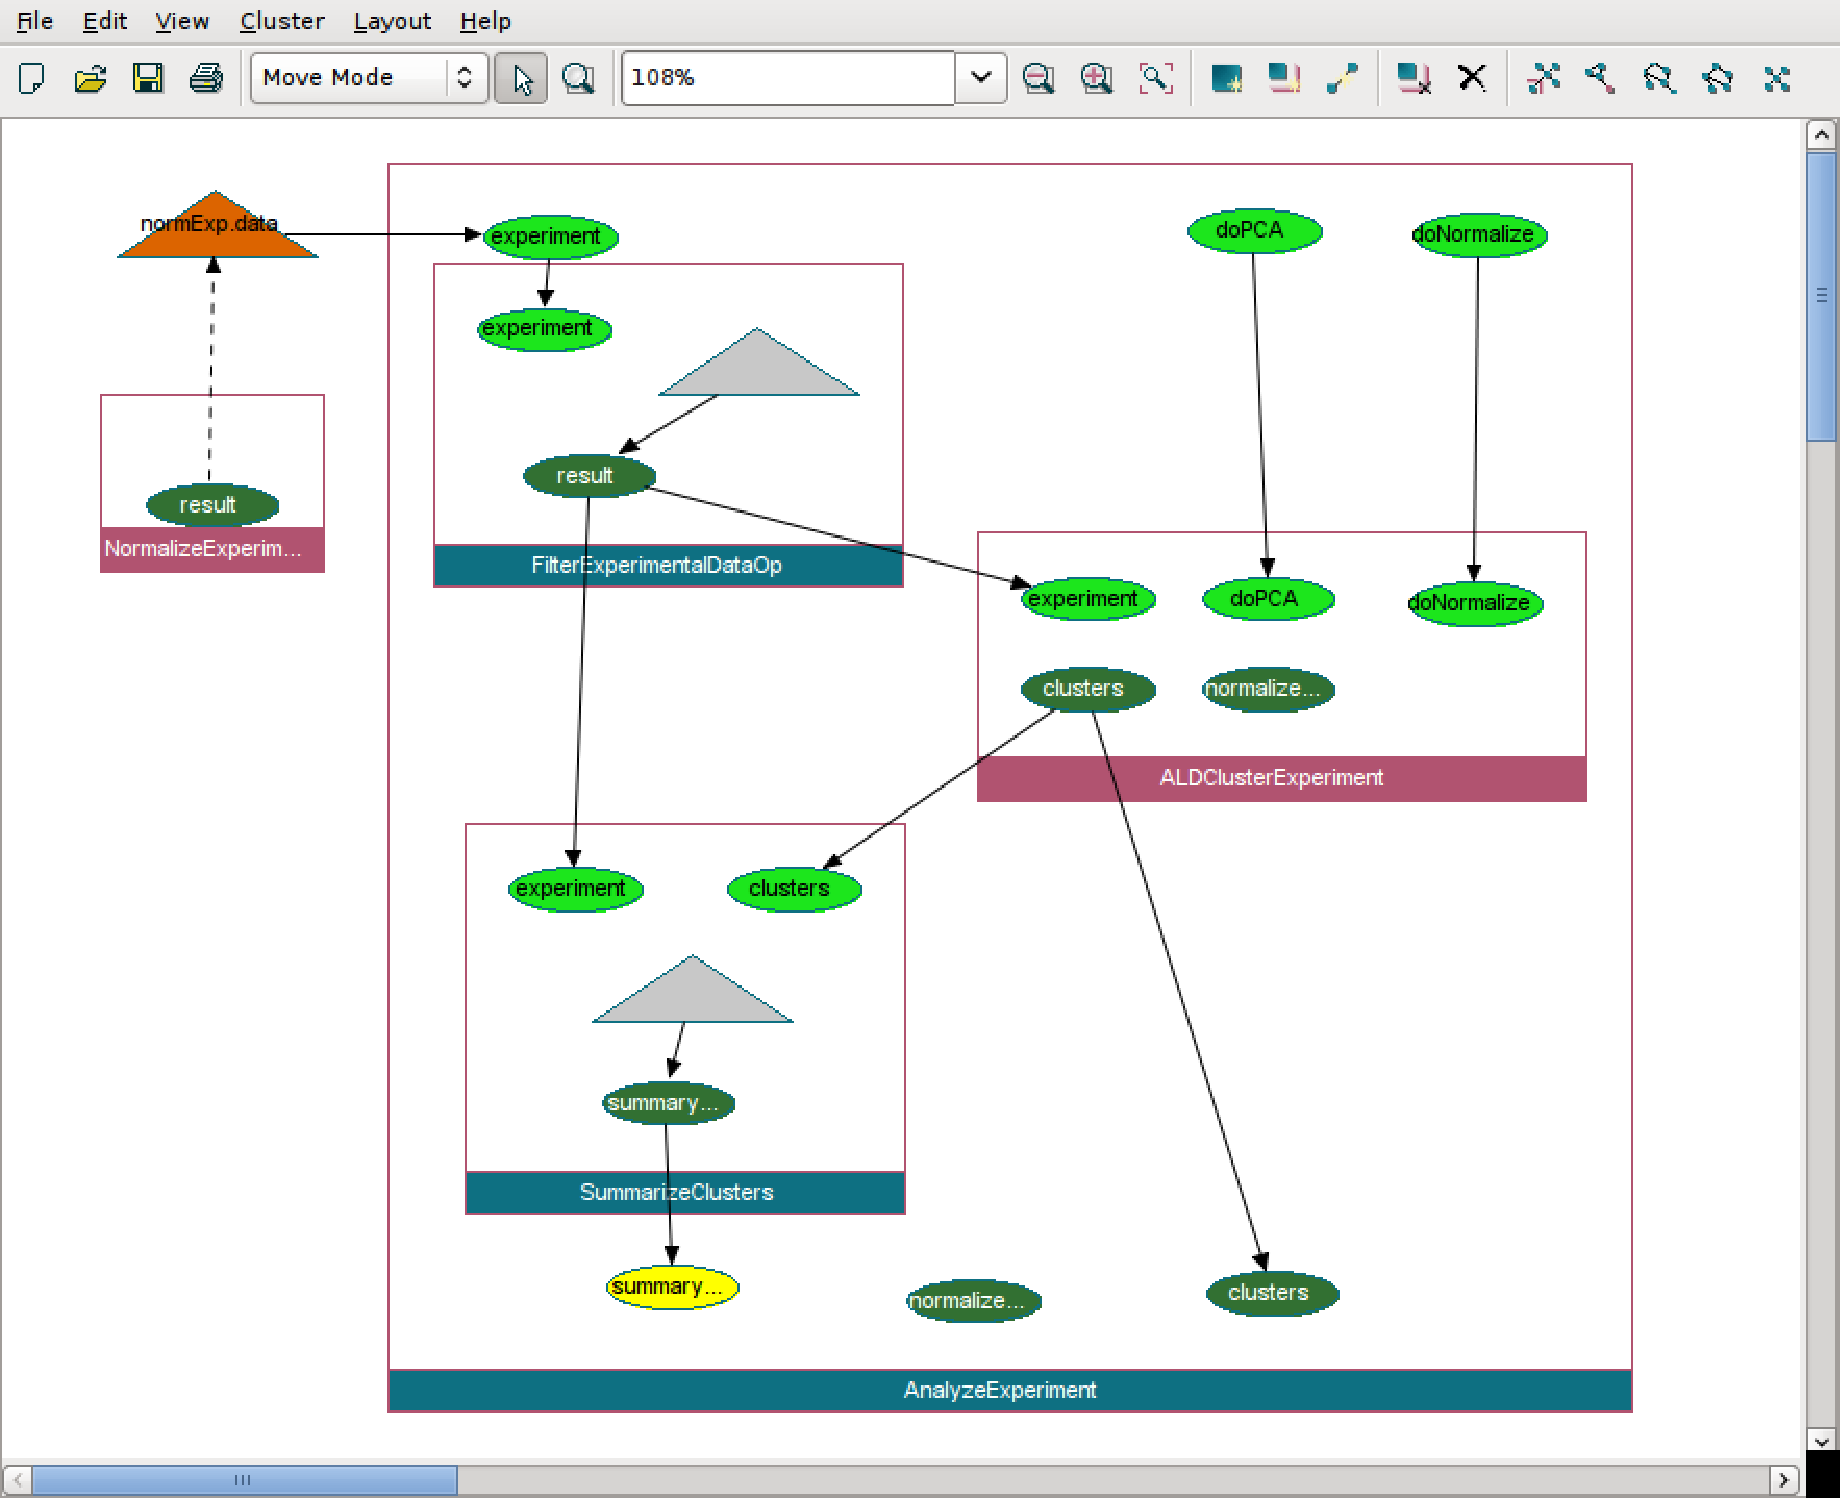
\includegraphics[clip, trim= 0 0 0 0, width=0.85\textwidth]{analyzeData-collapsed-edited}}}}
\caption[Example of a processing graph.]{\label{fig:DAG-repeat}
Example processing graph.
}
\end{figure}

\begin{figure}
\begin{center}
{\framebox{\includegraphics[clip, trim= 180 20 160 140, width=0.6\textwidth]{Exp1-correctedMaxima-txt-uncollapsed.png}}}
\caption{\label{fig:exa}Screenshot of \mtbc for a part of the same processing graph as shown in
Fig.~\ref{fig:DAG-repeat}, however, the collapsed instance of the
\icode{DetectBaseline1D} has been uncollapsed.}
\end{center}
\end{figure}

\subsection{Using \mtbc}

\mtbc is based on
{\em Chisio}, a free editing and layout tool for compound or hierarchically
structured graphs. In \mtbc all editing functionality was conserved, however, is not
required for inspecting a processing graph in virtually all cases.
{\em Chisio} offers several automatic layout algorithms where \mtbc chooses
the Sugiyama as default as this is most adequate for the hierarchical graph structure
of processing histories.
In the following we explain a tiny part of {\em Chisio's} functionality and the
extensions supplied by \mtbc.
For more details on {\em Chisio} see the User's manual of {\em Chisio} which is
included in the \mtbc package and also easily found in the web.

In Figure \ref{fig:DAG-repeat} an example processing graph extracted from a data analysis procedure
based on demo operators is shown.
As already described, 
instances of operators are depicted as rectangles, input and output ports as ellipses, and data ports as triangles.
All three types of elements of a processing graph are implemented as
{\em Chisio} nodes. A node may be selected with a left  or right mouse click.
A selected node may be dragged with the left mouse button pressed to manually adjust the
layout.
The size of a node representing operators is automatically adjusted to fit all enclosed
ports and nested operators.

The name of an operator is displayed in a colored area at the bottom of its rectangle.
If an operator node is uncollapsed it is shown in blue, if it is collapsed it is
of dark red.
This is shown in Fig.~\ref{fig:DAG-repeat} 
where the operator \icode{DetectBaseline1D}  
has been collapsed.
A selected operator node may be collapsed or uncollapsed 
via its context menu or by a left double mouse click while pressing down the shift key.
Collapsing makes all enclosed operator and data nodes invisible, thus, only
the ports of a collapsed operator are shown.
If the node is uncollapsed lateron, enclosed nodes are made recursively visible
again, until a collapsed node is encountered.
Uncollapsing additionally invokes the automatic layout algorithm, hence, any manual
layout adjustments applied before are lost.
If we uncollapse the operator \icode{DetectBaseline1D}
as shown in Fig.~\ref{fig:exa}, we can inspect the data processing 
accomplished within this operator.

If a data port represents data read from file,
the triangle is tagged by a string and colored orange.
%%If the
%%data object extends the class \icode{ALDData} this string gives the filename
%%the data was read from.
As the data read from file \icode{'Exp1-smooth.txt'}
has a processing graph associated,
this history is also included into the processing graph and 
connected by a dashed edge.
This history was written to the file \icode{'Exp1-smooth.txt.ald'} by previous
processing using \alida.

%%From this processing history we find
%%that the median operation has been applied to an image \icode{foo.pgm}
%%which in turn had no associated history.

\begin{figure}
\begin{center}
{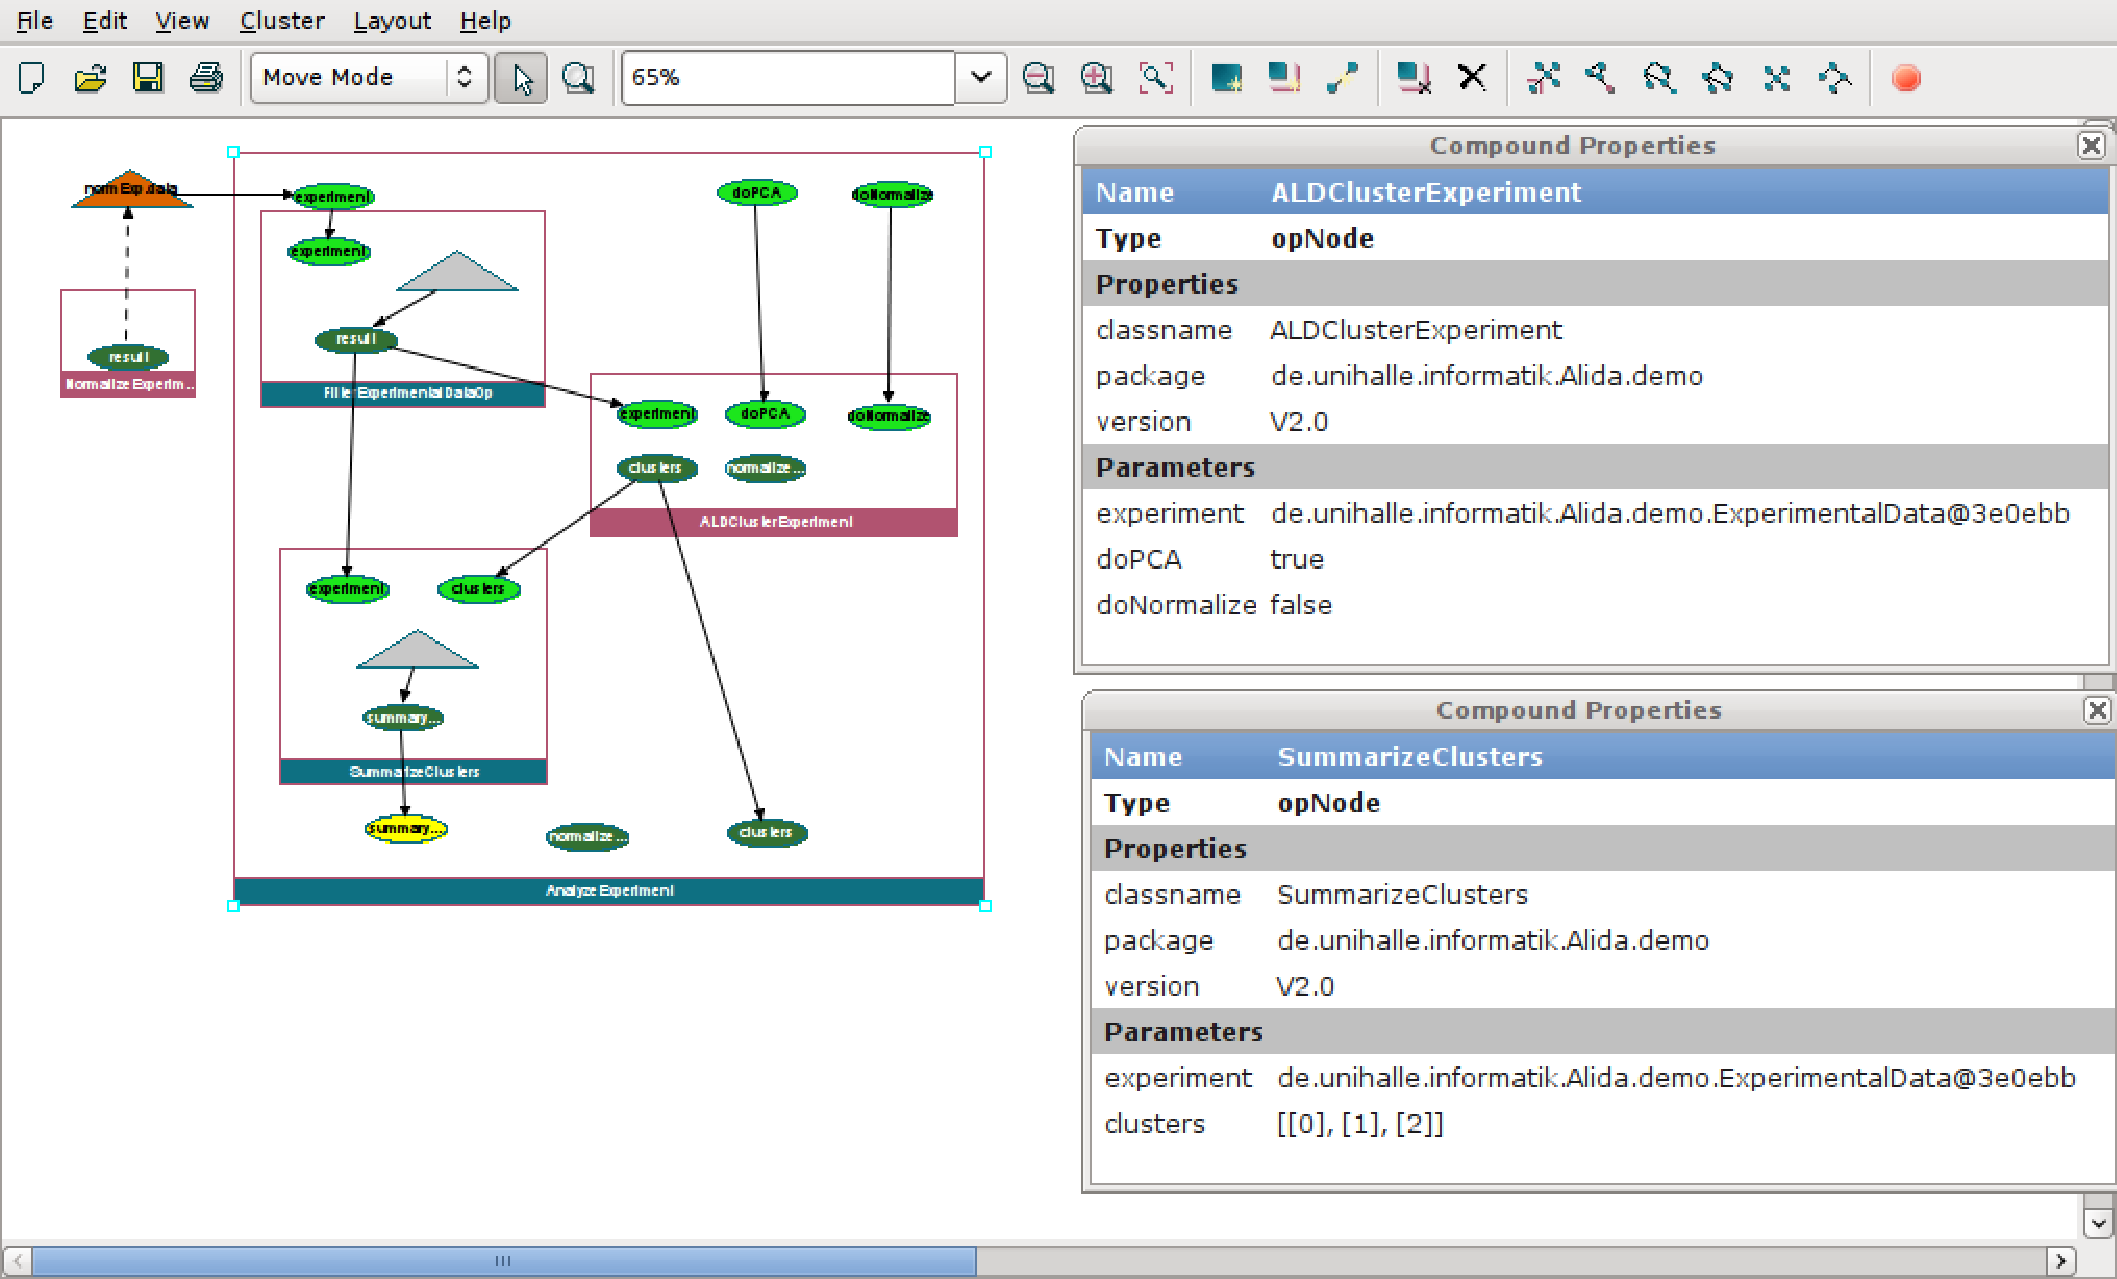
\includegraphics[width=\textwidth]{analyzeData-collapsed-edited-withProperties}}
\caption{\label{fig:exa1}Screenshot of \mtbc with details for the operators
\icode{SmoothData1D} and \icode{RefineLocalExtrema1D}.
}
\end{center}
\end{figure}


Input and output ports are generally displayed with light and 
dark green ellipses, respectively. 
The single exception
is the port for which the processing graph was constructed, which is depicted in
yellow.
In our example this is the output port \icode{'correctedExtrema'} of the
operator \icode{CorrectForBaseline1D}.

More details for operators and ports may be inspected using the \textit{Object properties}
of {\em Chisio's} nodes.
These are displayed in a separate window which
for the selected node can be popped up using the context menu.
The context menu is activated by a right mouse click.
Alternatively the object properties window can be popped up by a double left mouse click.

Information displayed includes:
\begin{itemize}\itemseparation{0.1em}
\item	name of the operator or port
\item	type of the node, e.g., \icode{opNode} for operators
\item	for operators the parameter values at time of invocation
\item	for input and output ports the Java class of the object as it was passed
into the operator along with the explanatory text of this port
\item	for output ports the properties of the object
	given when passed out of the operator, if it is of type \icode{ALDData}.
\end{itemize}
In Fig.~\ref{fig:exa1} this is shown for the operators
\icode{SmoothData1D} and \icode{RefineLocalExtrema1D}.




\end{appendix}

\end{document}

